\documentclass[11pt]{report}
\usepackage[utf8]{inputenc}
\usepackage[danish]{babel}
\usepackage [T1]{fontenc}
\usepackage[margin=2.5cm]{geometry}
\usepackage[hidelinks]{hyperref}
\usepackage{graphicx}
\graphicspath{{figures/}{Billeder/}}
\usepackage{listings}
\usepackage{color}
\usepackage{adjustbox}
\usepackage{tocloft}
\usepackage{listings}

\definecolor{dkgreen}{rgb}{0,0.6,0}
\definecolor{gray}{rgb}{0.5,0.5,0.5}
\definecolor{mauve}{rgb}{0.58,0,0.82}

\lstset{frame=tb,
  language=Java,
  aboveskip=3mm,
  belowskip=3mm,
  showstringspaces=false,
  columns=flexible,
  basicstyle={\small\ttfamily},
  numbers=none,
  numberstyle=\tiny\color{gray},
  keywordstyle=\color{blue},
  commentstyle=\color{dkgreen},
  stringstyle=\color{mauve},
  breaklines=true,
  breakatwhitespace=true,
  tabsize=3
}



\definecolor{bluekeywords}{rgb}{0.13,0.13,1}
\definecolor{greencomments}{rgb}{0,0.5,0}
\definecolor{turqusnumbers}{rgb}{0.17,0.57,0.69}
\definecolor{redstrings}{rgb}{0.5,0,0}

\lstdefinelanguage{FSharp}
                {morekeywords={let, new, match, with, rec, open, module, namespace, type, of, member, and, for, in, do, begin, end, fun, function, try, mutable, if, then, else},
    keywordstyle=\color{bluekeywords},
    sensitive=false,
    morecomment=[l][\color{greencomments}]{///},
    morecomment=[l][\color{greencomments}]{//},
    morecomment=[s][\color{greencomments}]{{(*}{*)}},
    morestring=[b]",
    stringstyle=\color{redstrings}
    }
\usepackage{amsmath}
\title{FogProjekt}

\author{
    Asger Hermind Sørensen\\
    cph-as466@cphbusiness.dk\\
    A klassen\\
    https://github.com/asgerhs\\
    https://157.230.110.215/FogProject \\
  &\\
    William Sehested Huusfeldt\\
    cph-wh106@cphbusiness.dk\\
    A klassen\\
    https://github.com/WSHuusfeldt\\
    http://138.68.77.14/FogProject 
  \and
    Andreas Vikke\\
    cph-av105@cphbusiness.dk\\
    A klassen\\
    https://github.com/AndreasVikke\\
    http://andreasvikke.dk/FogProject\\
  &\\
    Martin Eli Frederiksen\\
    cph-mf237@cphbusiness.dk\\
    A klassen\\
    https://github.com/Krigermus\\
    http://157.230.110.164/FogProject
  \and
\\\\
Projektet på git: https://github.com/asgerhs/FogProject \\
Java Docs: https://asgerhs.github.io/FogProject/HTML/apidocs/index.html\\
JaCoCo Code Coverage: https://asgerhs.github.io/FogProject/HTML/jacoco
\\\\
Afleveringsfrist d. 29/05-19.
}

\date{}

\begin{document}
\maketitle

\renewcommand{\cftchapleader}{\cftdotfill{\cftdotsep}}
\tableofcontents
\newpage

\chapter*{1. Indledning}
\addcontentsline{toc}{chapter}{1. Indledning}
Fog eksamensopgaven omhandler processen at gå fra planlægning til et
færdigudviklet administrationssystem for johannes fog. Under processen
har vi brugt forskellige redskaber til at opnå det færdige produkt som
bliver gennemgået i opgaven. Vi har brugt SCRUM som udviklingsmetode
hvilket har spillet en central rolle i vores projekt da projektet er
opbygget omkring denne udviklingsmetode. Vi har haft en product owner
tilknyttet projektet som vi i samarbejde med er blevet enige om
forskellige opgaver der skulle løses ugentligt. Disse opgaver har
været med til at bidrag til den samlede løsning af vores
færdigudviklede produkt.
\newpage


\chapter*{2. Baggrund}
\addcontentsline{toc}{chapter}{2. Baggrund}
\section*{2.1. Virksomheden}
\addcontentsline{toc}{section}{2.1. Virksomheden}
Fog har to afdelinger, hvor den ene afdeling er design og bolighus, og den anden afdeling er trælast og byggecenter. Denne rapport har arbejdet med afdelingen trælast og byggecenter. Der skulle udvikles et system for Fogs medarbejdere, således at de kunne se kunders forespørgsler på carporte, kontakte kunden, og hjælpe dem til at få bestilt den carport kunden ønsker. Således skulle medarbejderen kunne give kunden en pris samt en tegning over carporten med de korrekte mål. Til sidst ville medarbejderen kunne printe en stykliste over carporten og få sendt materialerne til kunden. 

\section*{2.2. Virksomhedens krav}
\addcontentsline{toc}{section}{2.2. Virksomhedens krav}
\begin{itemize}
\item\textit{Systemet skal give kunden mulighed for at bestille en carport ud fra kundens egne vilkårlige mål.}
\item\textit{ Kunden skal kunne få en stykliste med tilhørende tegning når
  forespørgslen først er sendt og en sælger har godkendt denne.}
\item\textit{ Sælgeren skal kunne ændre en forespørgsel efter en personlig samtale med kunden for at sikre at kunden ved præcist hvad han bestiller.}
\end{itemize}

\section*{2.3. Virksomhedens vision}
\addcontentsline{toc}{section}{2.3. Virksomhedens vision}
Fog skal have erstattet deres nuværende DOS system til noget nyt. Derfor vil Fog have udviklet et administrationssystem der giver dem og deres medarbejdere et større overblik og rigere mulighed for at kunne give deres kommende kunder præcis det de vil have. Med et bedre administrationssystem har Fog mulighed for at kunne give deres medarbejdere et kraftigt værktøj til både at øge salg, og gøre processen af et salg nemmere og mere effektivt. Systemet skal derudover også kunne effektivisere deres lagerstatus, således at lageret kan blive monitoreret, ændret og opdateret.  
\newpage

\chapter*{3. Sprog og programmer}
\addcontentsline{toc}{chapter}{3. Sprog og programmer}
\textbf{Loaklt:}
\begin{itemize}
  \item Windows - Linux - MacOS.
  \item Java v. 8.
  \item Mysql v. 8.0.14.
  \item MySQL Workbench v. 8.0.15.
  \item Github / Github Desktop.
  \item Netbeans v. 8.2.
  \item Maven v. 3.5.2.
  \item Taiga.io.
\end{itemize}
\textbf{Server:}
\begin{itemize}
  \item Linux - Ubuntu 18.10.
  \item Java Openjdk 11.
  \item Mysql v. 8.0.14.
  \item Maven v. 3.5.2.
\end{itemize}
\textbf{Diverse:}
\begin{itemize}
  \item Bootstrap v. 4.3.1
  \item jquery v. 3.4.1
\end{itemize}
\newpage

\chapter*{4. Domæne model og ER diagram}
\addcontentsline{toc}{chapter}{4. Domæne model og ER diagram}
\begin{center}
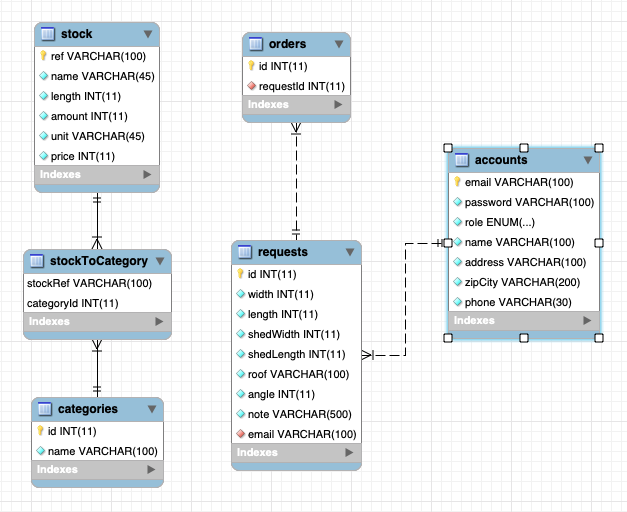
\includegraphics[width=11cm]{Er.png}
\end{center}
Databasen består af seks tabeller users, orders, requests, stock,
stockToCategory og categories. 
\\
\\
Accounts tabellen har username som
PRIMARY-KEY og har e-mail som UNIQUE, således at ingen af disse er
ens. Alle attributter er sat til at være NOT NULL. 
\\
\\
Requests tabellen har id som PRIMARY-KEY og er sat til
AUTO\_INCREMENT. Email attributten
er sat som Foreign Key til accounts på email. Alle attributter er sat
til at være NOT NULL. 
\\
\\
Orders tabellen har id som PRIMARY-KEY og er sat
til AUTO\_INCREMENT. requestId er sat som Foreign Key til requests på
id. Alle attributter er sat til at være NOT NULL. 
\\
\\
Stock tabellen har
ref som PRIMARY-KEY. Alle attributer er sat til at være NOT
NULL. 
\\
\\
stockToCategory tabellen har både stockRef og categoryId som
PRIMARY-KEY. Begge attributter er sat til NOT NULL. 
\\
\\
Categories tabellen har id som PRIMARY-KEY, og er sat til AUTO\_INCREMENT. Begge attributter er sat til NOT NULL.
\newpage

\chapter*{5. Navigations Diagrammer}
\addcontentsline{toc}{chapter}{5. Navigations Diagrammer}
Navigations diagrammet over hele systemet viser hvordan der kan navigeres rundt på hjemmesiden. Fra index.jsp kan man logge ind, registrere sig selv eller lave en forespørgsel på en carport. Hvis man er logget ind som kunde kan man også se sine forespørgsler, ens ordre og logge sig selv ud. Er man logget ind som admin kan man se alle forespørgsler, ændre forespørgsler, godkende forespørgsler og slette forespørgsler. Som admin kan man også se alle brugere, ændre deres rolle samt fjerne en bruger. Herudover kan man også se alle ordre og se deres styklister og tegninger. Er man logget ind som medarbejder kan man kun se, ændre, godkende og slette forespørgsler. \\
\begin{center}
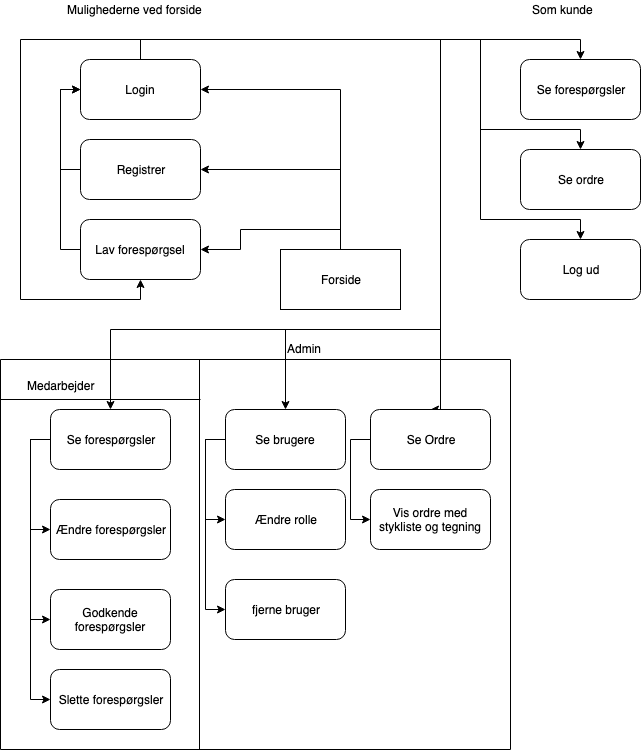
\includegraphics[width=12cm]{Overordnet.png}
\end{center}
Den første jsp side man som bruger kommer ind på er index.jsp, hvor man kan logge ind og registrere sig som bruger.
Har man ikke registreret sig gøres dette ved at trykke på ’Registrer’, hvor brugeren bliver henvist til register.jsp siden. Heri skal brugeren udfylde ønsket e-mail, adgangskode, navn, adresse, by og telefonnummer. Disse bliver brugt som parametre til at tilføje bruger når der trykkes på ’Opret’, hvor processen for at tilføje brugen til databasen starter. Brugerens rolle er pr. standard sat til at være ’Customer’. Brugeren bliver ikke tilføjet til databasen hvis e-mailen allerede er oprettet i databasen. Brugeren vil dermed få en fejlmeddelelse, som vises på siden og siger, at brugeren allerede eksisterer. Hvorefter brugeren skal indtaste oplysningerne på ny for succesfuldt at oprette sig.
Eksisterer brugeren ikke på forhånd bliver der vist en besked på siden om, at brugeren succesfuldt er blevet oprettet og man bliver redirectet til request.jsp siden.
Er der ikke behov for at oprette en ny bruger, skal vedkommende indtaste sin e-mail og adgangskode i de to felter og herefter trykke på ’Login’. Ved trykket bliver brugeren valideret, og sker dette succesfuldt vil brugeren blive logget ind. Er brugerens rolle enten ’Employee’ eller ’Admin’ redirectes brugeren til den respektive jsp side.
Er enten e-mailen eller adgangskoden indtastet forkert vises en fejlmeddelelse på siden, som informerer om dette. \\
\begin{center}
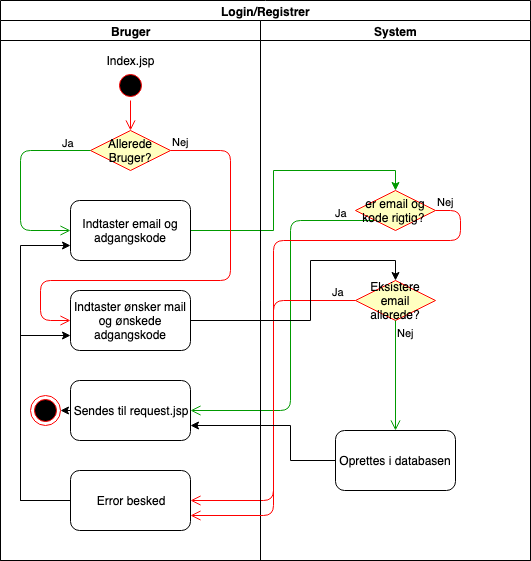
\includegraphics[width=14cm]{registrer.png}
\end{center}
Oprettelse af en forespørgsel. Kunden er inde på request.jsp og indtaster de påkrævet mål som er fremvist på siden, og derefter sender forespørgslen videre til databasen. En medarbejder henter forespørgslen fra databasen og ringer pågældende kunde op. Herfra sørger medarbejderen at kunden får præcis det som kunden ønsker, og kommer med eventuelle forslag til ændringer. Skulle kunden have nogle ændringer i sin forespørgsel ændre medarbejderen forespørgslen.
Til sidst når kunden er glad, bliver forespørgslen godkendt og sendt afsted som en ordre.
Skulle kunden vælge ikke at købe carporten sletter medarbejderen
forespørgslen fra databasen. \\
\begin{center}
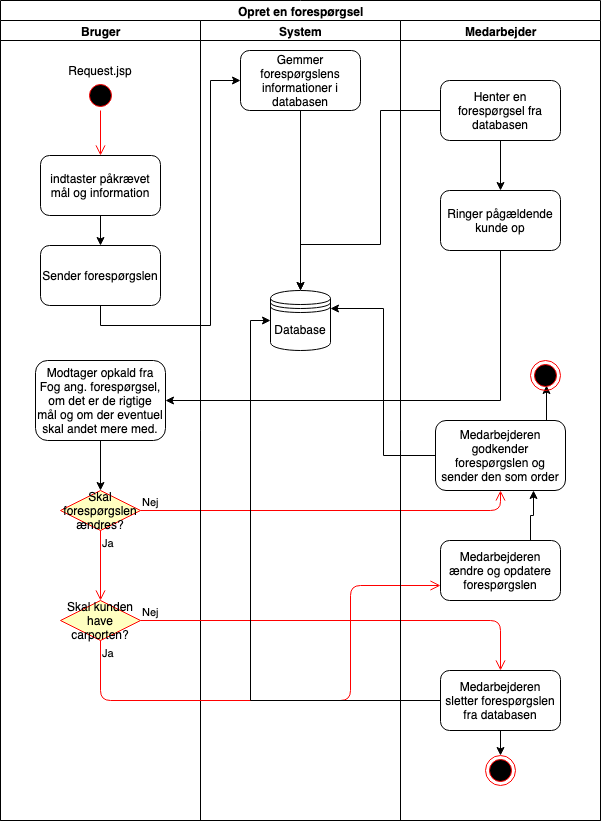
\includegraphics[width=13.5cm]{Foresporgsel.png}
\end{center}
Header området for brugere har fire knapper. Første knap fra venstre
er firma ikoner, der dirigerer brugeren til request.jsp, hvor der kan
laves en ny forespørgsel. Anden knap er lav forespørgsel, som gør det
samme som firma ikonet. Tredje knap er ordre, som dirigerer til
ordre.jsp, hvor brugeren kan se alle deres ordre. Sidste knap er log
ud knappen, som dirigerer til index.jsp. \\
\begin{center}
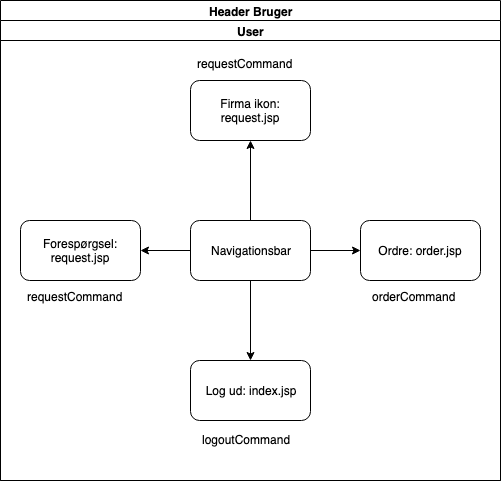
\includegraphics[width=8cm]{HeaderBruger.png}
\end{center}
Header området for en medarbejder har fire knapper. Første fra venstre
er firma ikonet, som dirigerer til requestList.jsp, hvor brugeren kan
se alle forespørgsler. Anden knap er lav forespørgsel der dirigerer
til request.jsp, hvor brugeren kan lave en forespørgsel. Tredje knap
er forespørgsels liste der dirigerer til requestList.jsp, hvor
brugeren kan se alle forespørgsler. Sidste knap er log ud, der
dirigerer til index.jsp. \\
\begin{center}
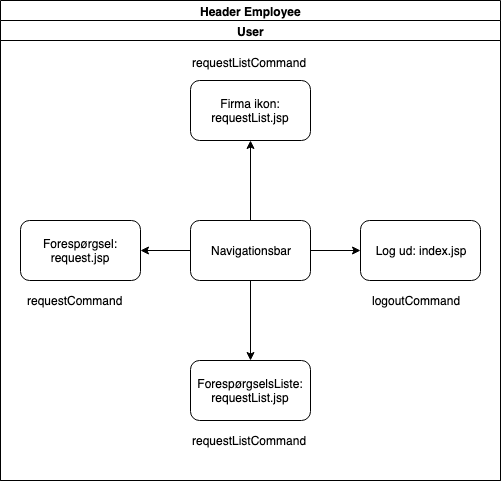
\includegraphics[width=8cm]{HeaderEmployee.png}
\end{center}
\newpage
\noindent Header området for admin har fire knapper. Første fra venstre er
firmaikonet, som dirigerer til requestList.jsp, hvor brugeren kan se
alle forespørgsler. Anden knap er forespørgselsliste, som dirigerer
til requestList.jsp, samme som firma ikonet. Tredje knap er ordre som
dirigerer til orders.jsp, hvor brugeren kan se alle ordre. Sidste knap
er log ud knappen som dirigerer til index.jsp. \\
\begin{center}
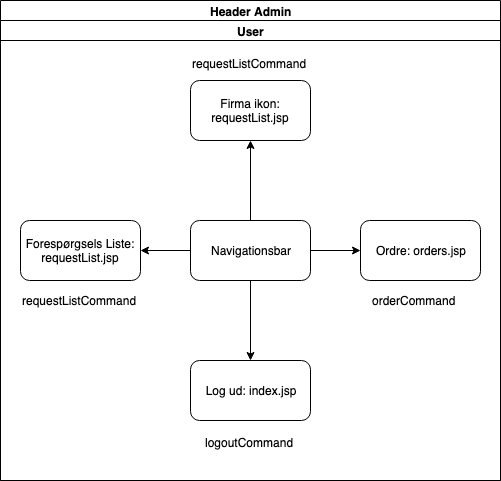
\includegraphics[width=8cm]{HeaderAdmin.png}
\end{center}
Brugere fanen for admin starter med at systemet henter alle brugere fra databasen. Admin kan derfra se alle brugerne og deres informationer. Hvis admin vil fjerne en bruger trykker admin på fjern bruger helt ude til højre for brugeren, og brugeren vil blive slettet fra databasen. Hvis admin gerne vil ændre en brugers rolle så trykker admin på en drop down menu der giver admin mulighed at ændre brugeren til enten kunde, medarbejder eller admin. Alt foregår på showUsers.jsp. \\
\begin{center}
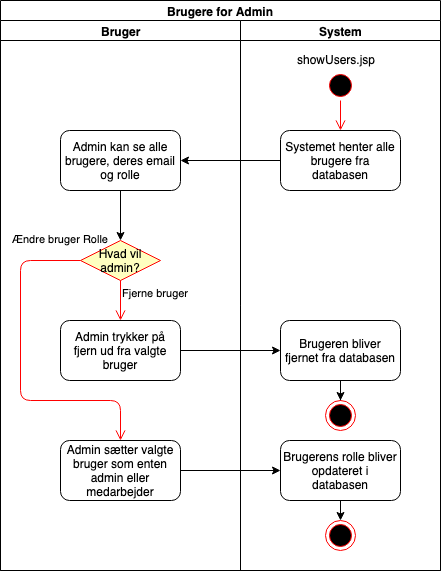
\includegraphics[width=7cm]{BrugereAdmin.png}
\end{center}
Ordre fanen for en bruger starter med at systemet henter alle brugerens ordre fra databasen. Herfra kan brugeren vælge at se en ordre ved at trykke på vis ordre, som dirigere brugeren til showparts.jsp igennem showPartsCommand, hvor brugeren derfra kan se styklisten for ordren samt en tegning over ordren. \\
\begin{center}
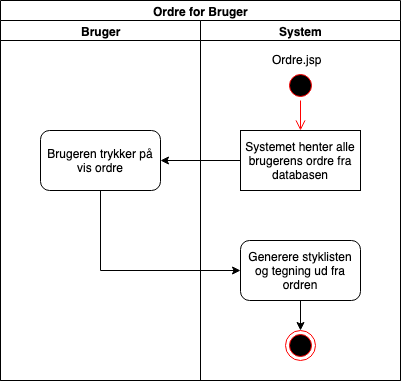
\includegraphics[width=9cm]{OrdreBruger.png}
\end{center}
Ordre fanen for admin starter på order.jsp, hvor systemet henter alle brugerne fra databasen. Herfra kan admin så vælge en ordre fra en pågældende bruger ved at trykke på vis ordre helt ude til højre for ordren. Herfra bliver admin dirigeret til showParts.jsp igennem showPartsCommand, hvor admin kan se styklisten for ordren samt tegningen der hører til den. \\
\begin{center}
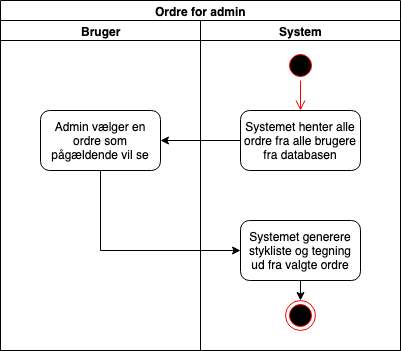
\includegraphics[width=9cm]{OrdreAdmin.png}
\end{center}
\newpage
\noindent Ved login som admin forwardes brugeren til showUsers.jsp. På denne jsp side henter systemet alle brugere fra accounts-tabellen i databasen. De bliver printet frem på siden i en liste. Herunder kan admin se informationer om den enkelte bruger – hvilken e-mail de er registreret med samt hvilken rolle de har. Her kan Admin træffe et valg om den enkelte bruger skal fjernes eller om rollen skal ændres. Som udgangspunkt bliver alle brugere oprettet som kunder i systemet, hvorefter Admin kan ændre en f.eks. nyansattes rolle til at være sælgere, hvorfor denne feature er implementeret. Hvis Admin ændrer brugerens rolle kaldes en metode gennem UpdateUserCommand. Metoden opdaterer brugerens rolle i databasen og brugerens rettigheder ændres hermed også.
Vælger Admin at fjerne en bruger gøres dette ved at markere en bruger og trykke på ’Fjern’, en metode eksekveres gennem showUsersCommand klassen og sletter brugeren fra account-tabellen. \\
\begin{center}
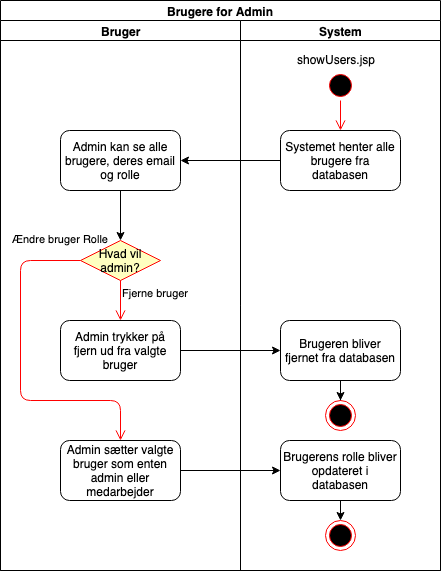
\includegraphics[width=13.5cm]{BrugereAdmin.png}
\end{center}
Hjemmesiden giver også mulighed for Admin og sælgere at se alle forespørgsler i databasen. Disse tilgås på requestList.jsp siden, hvor hjemmesiden viser en liste over dem alle. De er sorteret efter tidspunktet forespørgslerne er blevet oprettet på, den ældste forespørgsel vises derfor øverst. Brugeren har tre valgmuligheder for hver forespørgsel, disse værende henholdsvis at godkende forespørgslen, at opdatere den eller slette den.
Godkender brugeren forespørgslen trykkes der på knappen ’Godkend’. Ved trykket oprettes en ordre i databasen med forespørgslens id gennem RequestListCommand. Ordren oprettes dermed med dermed med dataen fra forespørgslen udelukkende baseret på dets id. Efter dette vil den ikke længere vises i listen over forespørgsler.
Ønsker brugeren i stedet at opdatere forespørgslen gøres dette ved at trykke på ’Rediger’, hvor brugeren redirectes til request.jsp siden, hvor forespørgslens oplysninger hentes gennem sessionen, som sættes gennem RequestCommand. Alle felterne vil derfor være udfyldt med dens nuværende oplysninger hvor brugeren her frit kan ændre på længde, bredde, skurets detaljer samt tagets detaljer. For at færdiggøre ændringerne trykkes der på ’Updates request’, som opdaterer forespørgslen med de nye værdier. Dette gøres gennem AddRequestCommand.
Vælger brugeren derimod at slette forespørgslen, skal der trykkes på ’Fjern’. Forespørgslen fjernes fra databasen og den vil ikke længere blive vist på listen. \\
\begin{center}
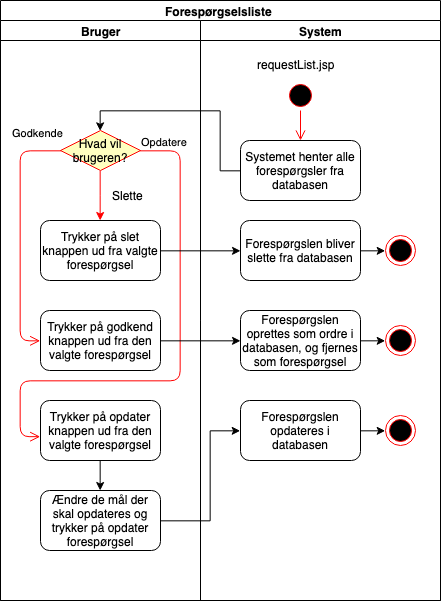
\includegraphics[width=11cm]{Foresporgselsliste.png}
\end{center}

\newpage

\chapter*{6. Sekvens diagrammer}
\addcontentsline{toc}{chapter}{6. Sekvens diagrammer}
\section*{6.1. Bruger}
\addcontentsline{toc}{section}{6.1. Bruger}
Forneden fremvises et sekvens diagram over en bruger der gerne vil købe en carport. Når en bruger gerne vil købe en carport så kan de fra forsiden (index.jsp) trykke sig videre til at bestille en carport uden at logge ind eller oprette sig. Dette sender dem videre til request.jsp igennem requestCommand. Herfra indtaster brugeren de krævede informationer, i bunden af formen indtaster brugeren informationer omkring sig selv, inkl en mail og password til at kunne komme ind og se deres bestilling. request.jsp validere derfra at formen er fyldt rigtigt ud når brugeren trykker på “send request”, er formen fyldt rigtigt ud så gemmes forespørgslen i databasen ved brug af add() metoden i requestMapper. 
Herfra venter brugeren på at en medarbejder kontakter dem, og spørger ind til carporten, og medarbejderen sørger for at brugeren får carporten som brugeren ønsker det, og lavet eventuelle ændringer skulle brugeren ønske det. 
Efter samtalen med medarbejderen blive forespørgslen godkendt, herfra
kan brugeren gå ind på index.jsp siden hvor brugeren logger ind, her
bliver e-mail og adgangskoden valideret af metoden validateUser()
gennem LoginCommand. Metoden instansieres som en boolean og dernæst
kører commanden et if-statement hvis boolean instansen af
validateUser() er true. Er dette tilfældet hentes brugeren fra
databasen gennem metoden getSingle() og sætter brugeren som attribut i
sessionen. Her bliver brugerens rolle fundet gennem en get-metode. Når
brugeren er logget ind kan brugeren nu se sin ordre under ordre fanen
i order.jsp.
\begin{center}
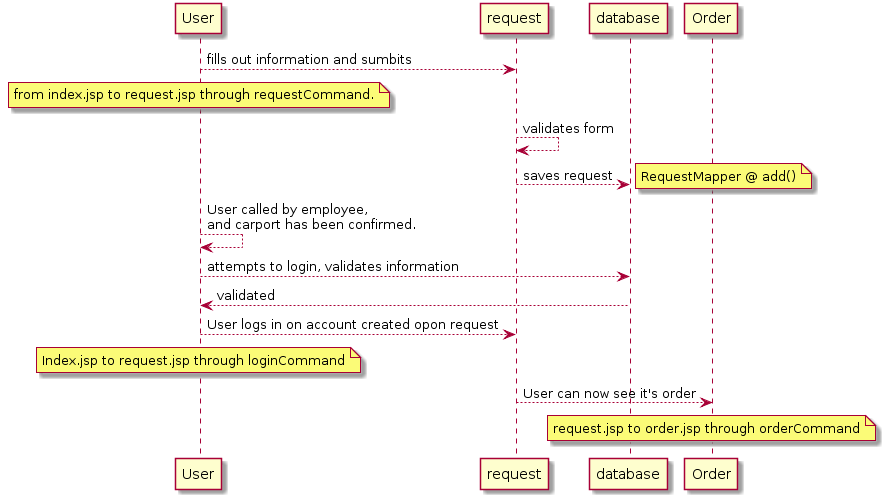
\includegraphics[width=15cm]{BrugerKob.png}
\end{center}
\newpage

\section*{6.2. Admin}
\addcontentsline{toc}{section}{6.2. Admin}
På index.jsp siden hvor brugeren logger ind bliver e-mail og adgangskoden valideret af metoden validateUser() gennem LoginCommand. Metoden instansieres som en boolean og dernæst kører commanden et if-statement hvis boolean instansen af validateUser() er true. Er dette tilfældet hentes brugeren fra databasen gennem metoden getSingle() og sætter brugeren som attribut i sessionen. Her bliver brugerens rolle fundet gennem en get-metode. Har brugeren en Admin rolle forwardes brugeren til requestList.jsp - hele denne proces gøres gennem LoginCommand.
Admin brugeren har flere rettigheder end en normal ’Employee’. Admin har adgang til at ændre brugernes rolle samt helt at fjerne brugeren. Admin skal her navigere til showUsers.jsp hvor listen af alle brugere i databasen vises. Skal en bruger opdateres til at være en ’Employee’ eller Admin gøres dette gennem UpdateUserCommand. Her henter commanden parametrene e-mail og rolle gennem request. Systemet tjekker efterfølgende om brugeren der logget ind er Admin ved at hente attributen fra brugeren gennem sessionen. Her er der inført et if-statement som tjekker om brugerens rolle er Admin. Er brugeren en Admin vil changeUserRole() metoden blive kørt og returnere en ny CommandTarget. Er brugeren ikke Admin vil der udelukkende returneres en ny CommandTarget og en fejlbesked.
Ligeledes kan en Admin også færdiggøre et salg af en carport som en medarbejder kan. 
\begin{center}
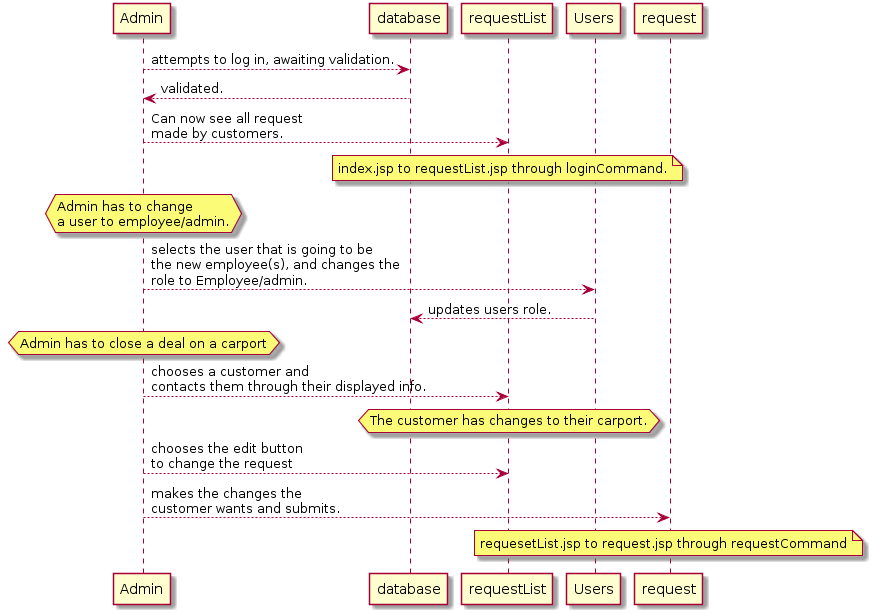
\includegraphics[width=15cm]{AdminArbejde.png}
\end{center}
\newpage

\section*{6.2. Medarbejder}
\addcontentsline{toc}{section}{6.2. Medarbejder}
En medarbejder adgang til at færdiggøre salg af carporte til kunder. På requestList.jsp siden kan medarbejderen se alle forespørgsler, hvor han her kan se detaljer for forespørgslen herunder også kontaktoplysningerne for kunden. Har kunden ønsker om at ændre forespørgslen kan medarbejderen også gøre dette. Brugeren forwardes til request.jsp siden for den valgte forespørgsel hvor dennes oplysninger hentes gennem sessionen hvis forespørgslens id ikke er null. Ellers vil der kastes en ny CommandException med en besked der fortæller, at forespørgslen ikke blev fundet.
RequestCommanden laver en ny forespørgsel og tjekker samtidig om det er en bruger der er logget ind eller ej, hvilket har betydning om brugeroplysningerne bliver hentet ned. Når det er en eksisterende forespørgsel som skal ændres, tjekker et if-statement om requestId er null, er den ikke det, sættes den nye forespørgsels ID til den der skal ændres. Metoden update() bliver kørt med den nye forespørgsels oplysninger, hvilket opdaterer forespørgslen i databasen.
Medarbejderen står til sidst med en forespørgsel præcis som kunden gerne vil have den. Forespørgslen godkendes og processen sættes i gang gennem RequestListCommand. Metoden består af et if-statement, som gennem request finder parametren for orderId, er dette ikke null vil statementet fortsætte. Et request objekt bliver instantieret ved et kald på metoden getSingle(), som henter en enkelt forespørgsel. Dette gøres på forespørgslens id og der bliver dermed oprettet en ny ordre med forespørgslens id ved brug af add() metoden. getAll() kaldes og henter alle forespørgsler og sætter dem som attribut i sessionen, her uden den nyligt oprettede ordre, som ikke længere er en forespørgsel.
Skulle det ske at kunden bakker ud af handlen, har medarbejderen mulighed for at slette forespørgslen. Ved et tryk på knappen ’Fjern’ kører RequestListCommandens else if-statement hvori metoden remove() kaldes på forespørgslen. Efterfølgende kaldes metoden getAll() og denne bliver sat som attribut i sessionen. Forespørgslen vil ikke længere vises på listen, eftersom denne er blevet fjernet fra databasen. 
\begin{center}
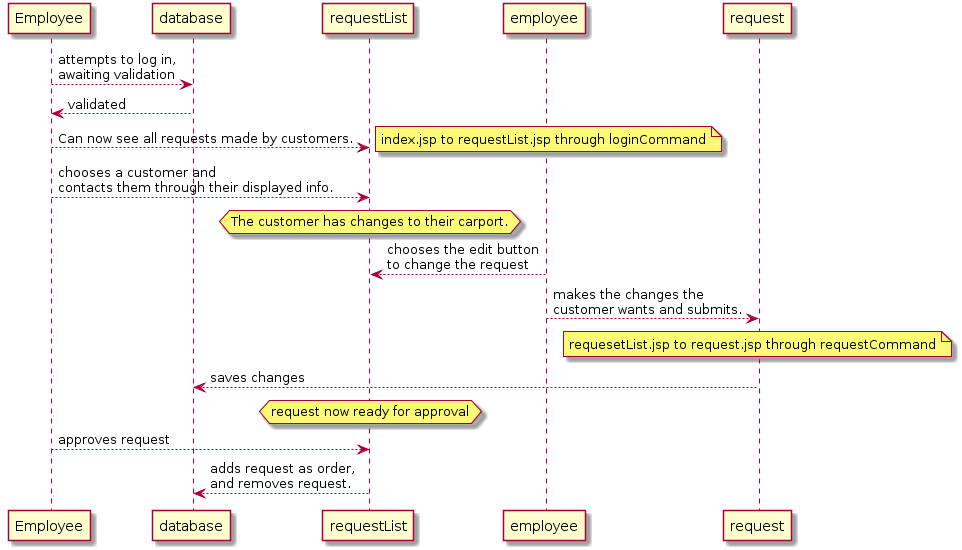
\includegraphics[width=15cm]{EmployeeArbejde.png}
\end{center}
\newpage

\chapter*{7. Særlige forhold}
\addcontentsline{toc}{chapter}{7. Særlige forhold}

\section*{7.1. Sessioner}
\addcontentsline{toc}{section}{7.1. Sessioner}
Session bliver brugt til at gemme data på tværs af flere side
forespørgsler. De har en udløbstid som gør at en bruger ikke bruger
for mange ressourcer over længere perioder. Til Fog projektet bliver
der gemt data der er hentet fra databasen og skal fremvises på
sitet. Når brugeren logger ind hentes brugeren f.eks. fra databasen og
gemmes i sessionen. Sider som OrderList, PartList, UserList og
RequestList henter lister af de tilsvarende data og gemmer i session
så JSP filerne kan tilgå dem og fremvise dem. \\\\

\section*{7.2. Håndtering af exceptions}
\addcontentsline{toc}{section}{7.2. Håndtering af exceptions}
Session bliver brugt til at gemme data på tværs af flere side
forespørgsler. De har en udløbstid som gør at en bruger ikke bruger
for mange ressourcer over længere perioder. Til Fog projektet bliver
der gemt data der er hentet fra databasen og skal fremvises på
sitet. Når brugeren logger ind hentes brugeren f.eks. fra databasen og
gemmes i sessionen. Sider som OrderList, PartList, UserList og
RequestList henter lister af de tilsvarende data og gemmer i session
så JSP filerne kan tilgå dem og fremvise dem. \\\\

\section*{7.3. Validering af brugerinput}
\addcontentsline{toc}{section}{7.3. Validering af brugerinput}
Alle input felter på sitet har en bestemt type som bestemmer hvad der
kan skrives i input feltet. F.eks. Nummer felter har typen
\textit{“number”} og password har typen \textit{“password”}. Dette gør
at der ikke kan skrives bogstaver i et tal felt osv. I alle servlets
har vi en try catch der vil catche hvis et input felt har en værdi den
ikke burde have og sende en error besked tilbage til brugeren. På den
måde er vi sikre på at vi skriver de rigtige værdier ned i databasen.
\newpage

\section*{7.4. Sikkerhed ved login}
\addcontentsline{toc}{section}{7.4. Sikkerhed ved login}
Projektet har 3 bruger grupper, Customer, Employee og Admin. Customer
er standard gruppen, som alle der opretter sig på siden bliver
tildelt. Gruppen har adgang til at oprette en forespørgsel på en
carport og se sine tidligere ordre. Employee gruppen kan blive tildelt
til brugere af en admin. Gruppe har adgang til at oprette
forespørgsler og se, redigere og godkende forespørgsler. Admin gruppen
er den højeste gruppe og har adgang til alt de andre grupper har, men
har også adgang til en bruger liste, hvor man kan ændre gruppen på
brugere, og en ordre liste. Når en bruger logger ind, bliver email og
passwordet sendt til serveren, hvorefter serveren kryptere passwordet
for at se om det matcher det hashede password der ligger i
databasen. Krypteringen der bliver brugt kaldes MD5, og bliver lavet
gennem klassen MessageDigest fra java.security. Krypteringen bliver
lavet for ikke at gemme plain tekst passwords i databasen, på den måde
kan password’sne ikke læses med det blotte øje. \\\\

\section*{7.5. MySQL Brugertyper}
\addcontentsline{toc}{section}{7.5. MySQL Brugertyper}
MySQL databasen har 3 brugertyper, root, transformer og reader. De lokale database connections gør brug af root som har adgang til alt. Da root har adgang til alt er det nemt at opsætte både test og normale skemaer, samt tabeller uden at skulle give adgang til dem. På live versionen bruges brugertypen transformer og reader. Transformer bliver brugt i alle tilfælde hvor der skal tilføjes, opdateres eller fjernes noget fra databasen. Reader bliver brugt når der skal læses fra tabeller. Transformer og reader har derfor kun adgang til det ene skema som der tilhører projektet.
\newpage

\chapter*{8. Udvalgte kodeeksempler}
\addcontentsline{toc}{chapter}{8. Udvalgte kodeeksempler}
\section*{8.1. Ajax Fil}
\addcontentsline{toc}{section}{8.1. Ajax Fil}
\begin{lstlisting}
$(document).ready(function() {
    $("#ajaxForm").submit(function (e) {
        e.preventDefault();
        ajax($(this));
    });
});

// Ajax Command
function ajax(formObj) {
    $.ajax({
        url: $(formObj).find('button').attr('formaction'),
        data: $(formObj).serialize()
    }).done(function (data, textStatus, request) {
        if (request.getResponseHeader('redirect') !== null) {
            window.location = request.getResponseHeader('redirect');
        }
        else if (request.getResponseHeader('error') !== null) {
            $("#errorBox #message").html(request.getResponseHeader('message'));
            $("#errorBox").show();
            $("#successBox").hide();
        } else {
            $("#successBox").html(request.getResponseHeader('message'));
            $("#successBox").show();
            $("#errorBox").hide();
        }
    });
}
\end{lstlisting}
Kode eksemplet ovenfor er fra filen ajax.js der ligger i mappen JS under Web Pages. Koden starter med et event som spørger om websitet er loaded, efterfulgt af en opsætning af endnu et event. Det nye event bliver sat til at lytte på alle forms som har id’et “ajaxForm” og hvornår de bliver indsendt. Når formene bliver indsendt vil eventet opfange det og køre den første linje i funktionen som hedder “preventDefault”. Denne metode gør at formen ikke bliver indsendt på normal vis gennem HTML, i stedet kaldes metoden ajax. Ajax metoden modtager selve formen hvor alle input felter og formactionen befinder sig.
jQuery har en indbygget metode som kaldes ajax, denne metode bruges til at udveksle data mellem klienten og serveren uden at opdatere siden. Ajax metoden modtager 2 væsentlige ting, url og data. Url er hvor forespørgslen skal sendes hen, i dette tilfælde skal den sende det til formactionen som er tilknyttet knappen i formen. Dataen er de parameter som skal sendes til severen. Her bruges metoden serialize fra jQuery som udpakker formen og bruger alle input felterne som parameter til urlen. 
Efter Ajax har sendt dataen til urlen, vil den få et svar tilbage fra
serveren. Derfor sættes et event op som kaldes “done”.  I done eventet
kan der gøres mange forskellige ting, i dette projekt er done eventet
brugt til at omdirigere til en ny side, udskrive en fejl besked eller
en succes besked. Omdirigering fungere ved at sætte sitets location
til “redirect” parameteren i headeren hvis den er sat. Beskederne
bliver vist ved at tilføje beskeden til elementet gennem jQuerys html
metode, hvorefter metoderne show og hide bliver brugt til at vise og
skjule boksene. \\\\

\section*{8.2. Mapper Interface}
\addcontentsline{toc}{section}{8.2. Mapper Interface}
\begin{lstlisting}
public interface MapperInterface <T, S> {
    List<T> getAll() throws Exception;
    T getSingle(S s) throws Exception;
    void add(T t) throws Exception;
}

public class MaterialMapper implements MapperInterface<Material, String> {}
\end{lstlisting}
Projektets mappers bruger alle det samme universale interface som har tre metoder. Hver mapper returnere sit eget objekt i form af modeller, RequestMapper returnere f.eks. modellen Request. Eftersom de returnere forskellige objekter er interface bygget med Java Generics, som gør det muligt at definere hvilket objekt der skal bruges når interfaces bliver implementeret. Samtidig bruger interfaces også et andet objekt til getSingle metoden. Grunden til dette er at mapperne har forskellige typer til getSingle. MaterialMapperen henter data fra databasen hvor primary key er en Streng, men ReuqestMapperen bruger en Integer som primary key.
\newpage
\chapter*{9. Status på implementation}
\addcontentsline{toc}{chapter}{9. Status på implementation}
Vi har primært opfyldt de ønskede implementationer med et par enkelte mangler. Vores tanke i helhed var at lave en så uafhængig stykliste beregner som muligt men kom kun halvvejs i mål med dette. Uafhængig i form af at den skal kunne modtage de relevante oplysninger fra vores database i forhold til de materialer der er til rådighed. Det at vi kun kom halvvejs i mål med dette vil sige at vores stykliste beregner tager højde for lagerstatus i forhold til længder på det tilgængelige træ, men tager ikke højde for lagerstatus af fx bolte og skruer. Det var ikke muligt for os at gennemskue en ordentlig løsning til hvordan vores beregner skulle skelne en bestemt skrue fra en anden skrue idet der ikke var den store mening i at definere en skure på baggrund af den længde. Derfor kunne vi ikke opnå vores ønskede resultat men i stedet antager vi at der kun findes bestemte slags skruer og bolte som bliver brugt i alle sammenhæng. Vi overvejede en løsning hvor det var muligt at se på fx størrelsen af skrue pakker og tage den pakke der passede bedst størrelsesmæssigt. Vi valgte så at gå lidt væk fra dette igen da der så også kunne være forskellige størrelse på skruerne i disse skrue pakker. Vi mangler også at implementere muligheden for at en ansat kan tilføje et materiale til vores database/lagerstatus så vores stykliste beregner kan tage højde for denne. Dette er mere eller mindre ligetil men vi fik disponeret vores tid lidt forkert da vi brugte ret meget tid på stykliste beregneren og nåede så ikke at implementere hele vores idé. Det er set i bakspejlet ikke særlig smart at lave en beregner der kan noget bestemt og så ikke kunne give den muligheden for at gøre det vi har kodet den til at kunne.


Vi nåede heller ikke at sikre vores visning af en ordre imod at en
bruger går op i urlen og skriver at de gerne vil have en ordre med et
andet id. I vores url nu kan man ikke se at der bliver sendt et id med
for at få en ordre men det bliver sendt med som en skjult parameter og
derved kan man også bare gå op i urlen og selv angive parameteren og
derved få en ordre der egentlig ikke er ens egen. Dette kunne være
løst ved at sikre at den bruger vi har gemt i vores session faktisk er
den korrekte bruger til den ordre brugeren gerne vil se. Altså en
simpel if statement.\\

\begin{center}
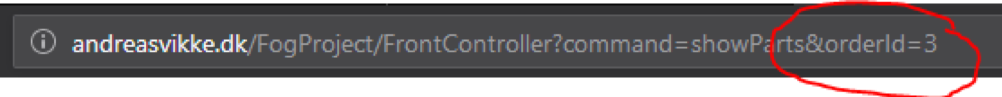
\includegraphics[width=15cm]{Picture1.png}
\end{center}

Vi havde også en plan om at få lavet en svag hvor man kunne se
hældningen forfra med de givne mål for en carport med rejsning. Da vi
først skulle til at lave svg’er med hældning begyndte de at drille
lidt så vi fik kun lavet de allerede eksisterende svg’er om sådan at
de passede til en carport med hældning. På de nuværende svg’er kan man
så se at der er kommet lægter ovenpå de spær der allerede var på
tegningen.
\newpage

\noindent Vores PO påpegede ikke noget om at vi skulle give en kunde mulighed for at se en en tegning over sin carport før vedkommende bestiller den. Vi ser det lidt som et problem da kunden så ikke får lov til at se om det faktisk er det kunden forventer og derfor var det en ting vi godt ville have lavet men som vi ikke nåede. Det vil give god mening at kunden kunne få lov til dette men vores fokus var et andet sted i opgaven og da vores PO ikke lagde vægt på dette var det en ting vi ikke tænkte over før i sidste øjeblik. Vi giver heller ikke kunden muligheden for at se prisen over den carport kunden er ved at bestille før kunden acceptere tilbuddet hvilket egentlig også burde være lavet så kunden får mulighed for at se om det overskrider kundens budget. Igen var det ikke noget PO lagde vægt på så det var endnu en ting vi først tænkte over meget sent og fik derfor ikke implementeret dette.

\newpage

\chapter*{10. SCRUM}
\addcontentsline{toc}{chapter}{10. SCRUM}
Scrum er en agil udviklingsmetode baseret på en trinvis tilgang og med stor vægt på projektledelse. Disse trins varighed er typisk to til fire uger, de kaldes sprint og gør hyppigt brug af feedback fra slutbrugeren, eller product owner. Udviklingsmetoden er især agil idet den giver mulighed for ændringer undervejs, hvorfor netop inddragelsen af slutbrugeren er særligt vigtigt. Scrum er dermed også organiseret da denne skal dokumenteres undervejs ud fra en prioriteret backlog, hvis indhold skal godkendes af product owner eller slutbrugeren. Hver iteration er fungerende del af produktet.

Daily Scrum møder var med til at give alle gruppemedlemmer et indblik i hvad der blev lavet, og hvad der skulle laves. Møderne er korte men meget essentielle. Dette gav gruppen en god oversigt opgaverne, og var stor hjælp til at undgå forvirring i blandt gruppen. 

Sprint planning sker sammen med pågældende produkt indehaver. Første Sprint planning bliver der aftalt med produkt indehaveren hvad der er en prioritet at få lavet først, og hvad der kan blive lagt i en backlog, til de næste sprints. Alle efterfølgende Sprint planning skal der kunne demonstreres noget for produkt indehaveren fra det sprint der er gået, og nye user stories fra backloggen sættes i prioritet og sættes ind til det næste sprint. 

Scrum masteren er den der holder styr på et sprint, sørger for at gruppemedlemmerne laver de rigtige ting, og indkalder til Daily Scrum møder. Når en opgave er løst går man til Scrum masteren og spørger om hvad pågældende person gerne vil have der skal laves. 

Scrum masteren blev roteret hver uge, således at alle var scrum master igennem hele forløbet. Dette var en god måde for hele gruppen, således at alle fik prøvet at være det. På denne måde blev der også fundet styrker og svagheder i blandt gruppens medlemmer. \\\\

\section*{10.1. Scrum Retrospective}
\addcontentsline{toc}{section}{10.1. Scrum Retrospective}
For hvert sprint møde med enten PO eller teknisk vejleder, var udgangspunktet for gruppen at få afklaret spørgsmål der havde kumuleret i løbet af sprintet.
Sprint mødederne med den tekniske vejleder gav rådgivning hovedsageligt på at rydde op i koden og gøre den mere letlæselig. Blandt andet rådgivning vedrørende SVG tegningerne der skulle genereres, her mente vejlederen at det ville være en god idé at skrive koden i Java og lade denne generere et SVG tag i HTML frem for direkte at skrive det i HTML.

Møderne med product owner var de mest givende. PO kunne klargøre
usikkerheder der havde hobet sig op i løbet af de enkelte sprint,
hovedsageligt ved besvarelse af de spørgsmål der måtte
forekomme. Disse møder gav klarhed til at arbejde videre med idéer
gruppen havde, men også at efterlade idéer som PO dømte irrelevante. \\\\
\section*{d. 16/5 - Møde med PO}
Til mødet blev det fremlagt, at databasen gerne skulle ombygges for at
fungere optimalt med den vision både udvikler holdet og PO havde for
produktet. PO ville selvfølgelig gerne have en database der fungerer
perfekt med systemet, men kritiserede tidspunktet for ombygningen af
den. PO ønskede at se User Stories for ombygningen og spurgte
efterfølgende ind til, hvad den kommende uge skulle gå på. PO bad om
flere User Stories, som dokumentation for den kommende uges
arbejde. Det blev aftalt, at databasen skulle færdiggøres og at
systemet skulle finpudses. \\\\

\section*{10.2. Scrum User Stories}
\addcontentsline{toc}{section}{10.2. Scrum User Stories}
Projektet består af 15 user stories, som er udarbejdet af gruppen og godkendt under møderne med PO. De første user stories der blev fremlagt for PO var ikke alle godkendte, PO ville have at disse skulle være mindre og mere præcise.
Først og fremmest skulle nogle af user storiesne omhandle beregneren, disse blev opdelt i fire, PO ønskede at systemet skulle bygges i mindre dele frem for en enkelt stor. PO’s ønske og visionen bag systemet fordrede at der udover en beregner skulle være illustrationer af carporte. Dette blev tilføjet som user stories i mindre dele som det var med beregneren. Et andet ønske var også at man gennem hjemmesiden kunne lave en forespørgsel på en carport. Dermed skulle dette også indgå i user stories, her delt i eksempelvis at en medarbejder ønsker at se en liste over alle forespørgsler. User stories i dette projekt er dermed bygget op omkring de ønsker PO havde for systemet, det vil sige at hver del af funktionaliteten i systemet blev vist som en user story.
Hvad user storiesne ikke nødvendigvis omhandler er eksempelvis test af klasser. Dette forventes at være en aktiv del af systemet, eftersom hver user story består af et acceptans kriterium for hvilket bestemmer om en given user story anses som færdigudviklet. En vigtig pointe ved arbejde med user stories og sprint er, at hvert sprint skal være afsluttet, så alle user stories der ligger i et sprint skal være parat til at merges ind i master branchen. Det er vigtigt fordi der absolut ikke må tilføjes ufærdig funktionalitet til systemet.
\section*{Første Sprint}
\begin{itemize}
  \item \#12 som sælger, vil jeg gerne generer styklister for en carport med faste mål uden hældning og uden skur.
\end{itemize}
\section*{Andet Sprint}
\begin{itemize}
  \item \#7 Som medarbejder, vil jeg gerne kunne se en stykliste på en
    hjemmeside, med noget design.
  \item \#16 Som kunde, vil jeg gerne kunne lave en forespørgsel på en carport.
  \item \#10 Som kunde, vil jeg gerne kunne se en tegning over den carport jeg bestiller.
\end{itemize}
\newpage
\section*{Tredje Sprint}
\begin{itemize}
  \item \#13 som sælger, vil jeg gerne generer styklister for en carport med vilkårlige mål uden hældning og uden skur.
  \item \#14 som sælger, vil jeg gerne generer styklister for en carport med vilkårlige mål uden hældning og med skur.
  \item \#41 Som kunde vil jeg gerne kunne se en tegning over den carport jeg bestiller med skur.
  \item \#43 Som sælger vil jeg gerne kunne se en liste af forespørgsler.
  \item \#44 Som sælger vil jeg gerne kunne oprette en ordre ud fra en forespørgelse.
\end{itemize}
\section*{Fjerde Sprint}
\begin{itemize}
  \item \#17 Som medarbejder, vil jeg gerne kunne se pris for styklisten.
  \item \#15 som sælger, vil jeg gerne generer styklister for en carport med vilkårlige mål med hældning og med skur.
  \item \#42 Som sælger vil jeg gerne kunne se SVG med hældning på tag.
  \item \#53 Som kunde, skal jeg kunne have adgang til en brugervenlig hjemmeside.
\end{itemize}
\newpage

\chapter*{11. Test}
\addcontentsline{toc}{chapter}{11. Test}
Tests blev udført på alle mappers, facader og AdvanceCalculator. Mappernes metoder tilgår databasen på forskellige måder, de henter, opretter, opdatere og fjerner data. Derfor er det vigtig at sikre dataen er korrekt.
Når metoder henter data tjekker testen om det dataen stemmer overens med det forventede data. Og hvis der bliver tilføjet, opdateret eller fjernet noget tjekker testen om dataen er skrevet rigtigt ind i databasen.

Ved udførelse af test af AdvanceCalculator var det nødvendigt at teste sideeffekten af metoderne, da AdvancedCalculators opbygning består af void metoder. I forhold til andre klasser, kører alle metoderne i denne klasse i konstruktøren. Det var derfor nødvendigt at teste om en tilfældig stykliste fik tilføjet de rigtige antal materialer.

\begin{itemize}
\item AdvancedCalculator
\begin{itemize}
\renewcommand\labelitemi{--}
\item calcRackets()
\item calcPosts()
\item calcLathsRoof()
\item calcShedMisc()
\item calcBoltsAndSquares()
\end{itemize}
\item MaterialMapper / MaterialFacade
\begin{itemize}
\renewcommand\labelitemi{--}
\item getAll()
\item getSingle()
\item add()
\item getAllByCategory()
\end{itemize}
\item OrderMapper / OrderFacade
\begin{itemize}
\renewcommand\labelitemi{--}
\item getAll()
\item getSingle()
\item add()
\item getAllByCategory()
\end{itemize}
\newpage
\item RequestMapper / RequestFacade
\begin{itemize}
\renewcommand\labelitemi{--}
\item getAll()
\item getSingle()
\item add()
\item update()
\item remove()
\end{itemize}
\item UserMapper / UserFacade
\begin{itemize}
\renewcommand\labelitemi{--}
\item getAll()
\item getSingle()
\item add()
\item validateUser()
\item changePassword()
\item changeUserRole()
\item remove()
\end{itemize}
\end{itemize}
I projektet er der blevet installeret et plugin der hedder JaCoCo Code
Coverage. Dette plugin kan bruges til at se hvor meget af klasserne er
dækket af test. Som billedet viser nedenfor er alle metoderne i
mapperne dækket. Dog er der nogle manglede instruktioner, da vores
test ikke dækker alle catch metoder og hvad der sker i dem.
\begin{center}
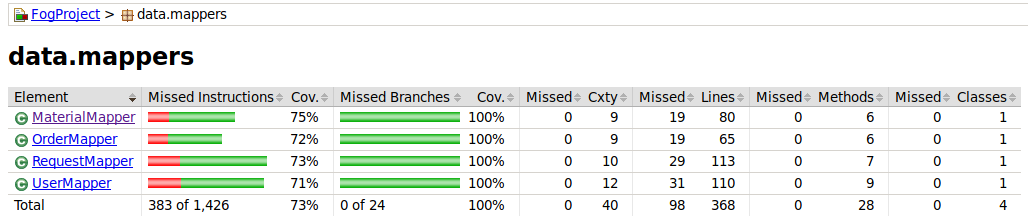
\includegraphics[width=15cm]{Test-Coverage.png}
\end{center}

\chapter*{12. Process}
\addcontentsline{toc}{chapter}{12. Process}
\textbf{Dette afsnit omhandler den arbejdsmæssige proces for at udvikle systemet. Delt op i to er hver del en vinkel på processen set fra et faktuelt synspunkt samt et reflekterende.}
\section*{12.1. Arbejdsprocessen faktuelt}
\addcontentsline{toc}{section}{12.1. Arbejdsprocessen faktuelt}
Der har i dette projekt været fem sprint med følgende størrelser:
\begin{itemize}
\renewcommand\labelitemi{--}
\item Første sprint, d. 23/4 - d. 26/4
User stories der er arbejdet med er \#12.
\item Andet sprint, d. 27/4 - d. 3/5 
User stories der er arbejdet med i dette sprint er \#7, \#10 og \#16.
\item Tredje sprint, d. 4/5 - d. 10/5
Dette sprint blev der arbejdet med user stories \#13, \#14, \#41, \#43 og \#44.
\item Fjerde sprint, d. 11/5 - d. 16/5
Sprintet bestod af user stories \#15, \#17, \#42 og \#53.
\item Femte sprint, d. 17/5 - d. 24/5
User stories var \#59 og \#60.
\end{itemize}
I alt har vi i gruppen arbejdet med 15 user stories fordelt på de fem sprints. Der blev taget højde for tidsestimatet af hver user story samt blev der er aftalt under møderne med PO hvilke af de fremlagte user stories der havde højeste prioritet.
Den user story som PO mente havde højeste prioritet skulle fremgå som den første i sprintet. Ydermere måtte gruppen ikke underpræstere og sætte for mange user stories på i et sprint og dermed ikke nå dem alle - alle user stories skulle være parate til mødet med PO. Derfor var det vigtigt at tage tidsestimatet i mente, da gruppen ellers ville have svært ved at færdiggøre sprintets user stories.
En vigtig pointe er, at tidsestimatet på user stories og dens prioritering ikke nødvendigvis har sammenhæng. Det kan dermed forekomme, at en user story med et relativ lavt tidsestimat har fået en højere prioritering end en user story med med et højere tidsestimat.
Strukturen af sprintenes længde er baseret på møderne med PO, det vil altså sige, at hvert sprints afslutningsdato er datoen for et møde med PO. Efter møderne påbegyndte det næste sprint, efter eventuelle rettelser af dets indhold i overenskomst med PO.
Grundet Scrums struktur og dens arbejdsproces, var det nødvendigt at
udvælge en scrum master, som skulle holde styr på holdets udvikling af
produktet. Eftersom projektet bestod af fire sprint eller mere blev
det muligt at skifte scrum master pr. sprint. Dermed arbejdede alle
gruppens medlemmer som scrum master i mindst ét sprint. Som
udgangspunkt delegerede scrum master user stories til medlemmerne og
fulgte op på hver user story’s udvikling. Det var ikke udelukkende
hele user stories som blev delegeret til medlemmerne. Der blev også
delegeret subtasks rundt, hvilket var mindre opgaver der skulle
udvikles for at den bestemte user story kunne anses som værende
færdig. Et eksempel kunne være user story \#43 “Som sælger, vil jeg
gerne kunne se en liste af forespørgsler”, hvilken bestod af tre
subtasks der skulle klares. \newpage
\noindent Subtaskene lød:
\begin{itemize}
\renewcommand\labelitemi{--}
\item \#46 Udskriv forespørgsler fra database til liste.
\item \#47 Udskriv liste på hjemmeside.
\item \#54 Opret dummy data til requests.
\end{itemize}
Hver subtask har også et tidsestimat her henholdsvis 2, 4 og 1 time. Skulle et enkelt medlem lave hele user story’en eller skulle den deles op, så et enkelt medlem tog en subtask, dette var op til scrum master.
I de fjerde sprint valgte scrum master at delegere user stories ud på baggrund af medlemmets arbejde i tidligere sprint, for at give et eksempel blev user story \#15 delegeret til to medlemmer, hvoraf den ene havde en mere rådgivende rolle. Den rådgivende partner havde arbejdet med tidligere user stories omhandlende beregneren i produktet.
Ligeledes blev det bestemt af scrum master i første sprint, at medlemmet med den stærkeste matematiske baggrund skulle tage styringen af user story \#12, for hvilken blev prioriteret højest af PO.
I løbet af hvert sprint kumulerede spørgsmål til produktets identitet, hvilken retning skulle det tage? Hvad blev anset af PO som værende vigtigst?
Spørgsmålene var både bred såvel som de var præciserede. Under et sprint var hovedspørgsmålet som gruppen ville have svar på, måtte gruppen lave antagelser? Dette kunne uddybes ved udviklingen af beregneren, hvor vi i gruppen blev nødt til at begrænse arbejdet på denne. Det var uvist om udviklingen pegede i den rigtige retning, hvorfor der netop blev spurgt om det ovenstående. PO-møderne bestod hyppigst af spørgsmål og undren fra gruppen, hvilket blev der blev klargjort og svaret på af PO.
Det var ikke alle dage hvor gruppen valgte at mødes ved samme lokation og det havde en betydning for måderne hvorpå de dalge scrum møder blev afholdt. For de dage hvor gruppen valgte mødes samme sted blev der indkaldt til møde så snart alle gruppens medlemmer var til stede. Møderne blev dermed ikke afholdt på tider hvor der manglede medlemmer, dette blev prioriteret i sammenråd. På de dage hvor gruppen ikke havde mulighed for at være til stede samme sted faldt beslutning på at holde møderne et fast tidspunkt tidligt på dagen, hvor medlemmerne gennem en kommunikationstjeneste. Møderne varierede minimalt tidsmæssigt, men de blev holdt med en tidsbegrænsning på 10 min. - de forblev altså korte og præcise. Deres indhold gik på ny dagligt, her blev der oftest startet med en hurtig opsummering på hvor hvert medlem var med deres arbejdsopgave samt et tidsestimat på, hvor langt der var igen. Havde medlemmer behov for assistance blev der gjort plads til dette også.
Når et sprint var overstået blev der kaldt til et yderligere møde, oftest efter PO-møderne. Formålet var at gruppen skulle se i retrospekt på sprintet samt at kigge på det kommende sprint. 
Undervejs stødte gruppen på flere fejl begået tidligere. Disse fejl begrænsede fremdriften af udviklingen og blev nødt til at blive håndteret hurtigt. Det har betydet, at arbejdsprocessen ikke har fungeret perfekt, det har sløvet hastigheden og sået tvivl i, hvordan systemet skulle bygges op. Et eksempel på en sådan fejl var et medlem, som havde lavet en mapper på en måde der ikke kunne bruges som den skulle. Det blev derfor til en længere proces for et andet medlem, da denne skulle benytte sig af netop mapperen eftersom at mapperen og det nye kode ikke var kompatible.
\newpage

\section*{12.2. Arbejdsprocessen reflekteret}
\addcontentsline{toc}{section}{12.2. Arbejdsprocessen reflekteret}
\textbf{Dette afsnit består af gruppens refleksioner over
  arbejdsprocessen.}\\
Vi havde i gruppen ikke nogle problemer med scrum master rollen til at starte med, men i løbet af projektperioden blev rollen mindre og mindre betydende. Dette betød vel at mærke ikke at vi opgav rollen, tværtimod fortsatte vi gennem hele forløbet med at skifte scrum master hvert sprint. User stories blev også fint delegeret ud blandt medlemmerne i starten af hvert sprint. Med tiden begyndte vi i gruppen at påtage opgaverne på egen hånd, med mindre scrum masteren blev spurgt. 
Idéen om en scrum master er der ikke tvivl om godt kan fungerer, men det kræver en større indsats, hvilket bliver anerkendt af gruppens medlemmer. Scrum master bærer selvfølgelig det største ansvar, men de resterende medlemmer har også ansvar i at få det til at fungere. Vi rettede op på nogle af begynder fejlene, som vi var skyldige i at lave, hovedsageligt ved at søge mod scrum masteren for at gå i gang med nye subtasks eller user stories. Det tog dog længere tid at følge den rigtige tankegang i sådan en type fremgangsmåde.
Gruppens brug af scrum var derfor ikke perfekt, vi var prægede af småfejl i arbejdsprocessen, blandt andet blev de daglige scrum møder negligeret, vel at mærke ikke altid. Vi forsøgte at “stramme op”, men i retrospekt må det erkendes at indsatsen ikke var den højeste for netop disse. Det betød dog ikke at vi ikke dagligt blev ajour med hinandens arbejde. Vi har kommunikeret meget indbyrdes, snakket om problemer vi er stødt på undervejs. Vi søgte hjælp af hinanden og var generelt gode til at fortælle om de frustrationer vi måtte have.
Med hensyn til vores retrospektive møder blev disse nogle gange spredt ud over flere samtaler. Dette var heller ikke perfekt udført af os i gruppen. Men der blev snakket meget om PO-møderne efter de blev holdt, herunder svarende vi fik på de spørgsmål vi havde haft inden vi gik ind til mødet. Det var hovedsageligt hvad vores retrospektive møder omhandlede, og det føltes også som om, at vi fik et bedre billede af hvad visionen med projektet var. Ofte var vi i tvivl om, hvad PO helt præcist ville have, at systemet vi skulle udvikle til ham skulle indebære, eller hvad der var tilladt af os at udvikle.
Det er på baggrund af gode råd fra PO fra de første par møder med ham, at vi fik styr på hvilke user stories der skulle indgå i backloggen. Til at starte med havde vi fremlagt nogle stories der ifølge PO var alt for brede og vi blev nødt til at dele dem op. Så snart user stories var på plads kunne disse sorteres efter PO’s prioritering, herefter at fordele dem rundt. Fordelingen af vores user stories var ikke så meget et problem som det var en misforståelse, til at starte med. Efter noget rådgivning og snak, blev det lettere at forstå hvad der for PO var vigtigt i starten af forløbet og det vigtige i slutningen af forløbet. At bryde vores stories ned i subtasks var ikke just et problem, det faldt os relativt naturligt at f.eks. at vise alle forespørgsler på hjemmesiden, måtte der selvfølgelig være en tabel i en database, som skal have en forbindelse til Java projektet. Dertilhørende de forskellige klasser i projektet, hvilke metoder vi skulle lave, der skulle også kunne genereres dummy data til listen så vi kunne se det fungerede. Problemet opstod lidt, da udviklingen blandt medlemmerne ikke altid var konsekvent. Der kom nogle mindre afvigelser i koden, hvilket vi forsøgte at imødekomme ved i samråd at bestemme hvordan tingene skulle gøres.
Vores tidsestimering af vores user stories og de tilhørende subtasks afveg meget fra den reelle tid der blev brugt på dem. Vi besluttede i starten at vi hellere ville sætte mere tid af til en user story end for lidt, på denne måde ville vi oftere komme foran frem for at være bagud i vores sprint. Perfekt gik det ikke for ved sidste sprint kom vi bagud, da vi forsøgte os med en opgave der var for stor at færdiggøre inden for den tidsramme vi havde. Tilfredsstillende var det ikke, men lærerigt, det var det.
I gruppen har flere af samtalerne været præget af en undren over nogle af de tekniske møder. Følelsen i gruppen er, at disse ikke altid har været givende nok, og i nogle tilfælde har efterladt os med flere spørgsmål end vi kom ind med. Det har været spekuleret om grunden til den relativt passive vejledning har været på baggrund af materialet vi har kunnet vise frem under møderne. Vi har derimod også gået fra møderne med følelsen af, at vi har fået en del ud af det.
Der kom noget kritik på SVG i et af møderne, hvilket vi tog til os og ombyggede efter vejlederens anbefalinger. Dette følte vi var meget godt pointeret af vejlederen, for i retrospekt er den nye version lettere læsbart end det vi startede med at præsentere.
PO møderne er de møder hvor vi som gruppe har følt vi fik afklaret størstedelen af vores spørgsmål. Det er også disse møder hvor vores misforståelser er blevet klargjort af PO, hvorfor vi føler at disse også var lærerige. Vi har dog lagt mærke til, at der er afvigelser blandt de forskellige PO’er, eftersom vi en periode havde en substitut fra vores normale PO, men det var ikke noget problem for vores vedkommende. Møderne blev anset som gode og givende. De sørgede for at udviklingen ikke løb af sporet og tog en anden retning end den PO ønskede. Det blev vi også indforstået med hurtigt, at alle beslutninger ikke stod til os.
Vi havde en klar tilgang fra starten af, hvilket var, at vi helst så at alle medlemmer berørte alle dele af projektet. Vi ønskede ikke at gøre et medlem “ekspert” på et område af systemet, alle skulle have en hånd med inde over alt. Det var ikke ensbetydende med at vi alle skulle have lige stor del af hvert område, men blot at input og småting var påkrævet. Vi ville også gerne spille til vores styrker, eksempelvis som tidligere beskrevet i den faktuelle del, så fik medlemmet med mest matematisk erfaring styringen af beregneren. 
Det har fungeret på godt og ondt at have denne tilgang, specielt hvis man tager de fejl der blevet begået gennem forløbet i mente.
Som skrevet i den faktuelle del af dette afsnit, så stødte vi i gruppen på fejl der skulle udbedres. Her menes der vel at mærke ikke bugs, som systemet også var præget af under udviklingen. Der menes fejl i logikken, vi havde nogle steder bygget metoder op på en måde, der gjorde, at de ikke var kompatible med er andet medlems arbejde. Så frustrerende som det var lærte det os at vi i fremtiden skal koordinere vores arbejde bedre.

\begingroup
\renewcommand{\cleardoublepage}{}
\renewcommand{\clearpage}{}
\newpage
\chapter*{13. Bilag}
\addcontentsline{toc}{chapter}{13. Bilag}
\endgroup
\noindent

\section*{13.1. Sprint backlog}
\addcontentsline{toc}{section}{13.1. Sprint backlog}
Første Sprint\\
\textbf{\#12 Som sælger, vil jeg gerne generer styklister for en carport med faste mål uden hældning og uden skur.}\\
Størrelse: XXLarge\\
Acceptance kriterium: Skal beregne 100\% korrekt for mål uden hældning og skur.\\
Subtasks:
\begin{itemize}
\item \#18 Beregn stykliste for taget (12 timer).
\item \#19 Beregn stykliste for mål (12 timer).
\item \#20 Indsæt data i List (1 time).
\item \#28 Opret database/Opret lager tabel (1 time).
\item \#30 Indsæt dummy data (2 timer).
\item \#31 Datamappers (2 timer).
\item \#32 Database Connector (2 timer).
\item \#37 Print stykliste til terminal (1 time).
\end{itemize}
\leavevmode
\\
Andet Sprint\\
\textbf{\#7 Som medarbejder, vil jeg gerne kunne se en stykliste. }\\
Størrelse: Large \\
Acceptance kriterium: En korrekt stykliste skal kunne vises ved tryk på en knap.\\
Subtasks:
\begin{itemize}
\item \#21 Omskriv List til tabel output (2 timer).
\item \#23 Udskriv tabel på website (4 timer).
\end{itemize}
\textbf{\#10 Som kunde, vil jeg gerne kunne se en tegning over den
  carport jeg bestiller. }\\
Størrelse: Medium \\
Acceptance kriterium: Som kunde skal jeg kunne se en tegning før jeg
har bestilt min carport. Tegningen skal være dybere beskrivende og
hænge sammen med den som kunden bestiller.\\
Subtasks:
\begin{itemize}
\item \#39 Tegn top-down tegning af carport (4 timer).
\item \#40 Tegn side tegning af carport (4 timer).
\end{itemize}
\textbf{\#16 Som kunde, vil jeg gerne kunne lave en forespørgsel på en carport. }\\
Størrelse: Small \\
Acceptance kriterium: Kundes forespørgsel skal kunne sendes og ses af medarbejder. \\
Subtasks:
\begin{itemize}
\item \#33 Lav en form på hjemmesiden (2 timer).
\item \#38 Lav tabel i databasen til forespørgsler (2 timer).
\item \#36 Send forespørgelse til database (2 timer).
\end{itemize}
\leavevmode
\\
Tredje Sprint\\
\textbf{\#13 Som sælger, vil jeg gerne generer styklister for en carport med vilkårlige mål uden hældning og uden skur. }\\
Størrelse: Large\\
Acceptance kriterium: Skal beregne 100\% korrekt for mål uden hældning og skur. \\
Subtasks:
\begin{itemize}
\item \#24 Lav beregner for vilkårlige mål (10 timer).
\end{itemize}
\textbf{\#14 Som sælger, vil jeg gerne generer styklister for en carport med vilkårlige mål uden hældning og med skur. }\\
Størrelse: Medium\\
Acceptance kriterium: 100\% korrekt stykliste for skur.\\
Subtasks:
\begin{itemize}
\item \#27 Beregner for skur. (12 timer) .
\end{itemize}
\textbf{\#41 Som kunde vil jeg gerne kunne se en tegning over den carport jeg bestiller med skur. }\\
Størrelse: Medium\\
Acceptance kriterium: Tegning skal kunne vise præcist hvor stolper osv. skal placeres.\\
Subtasks:
\begin{itemize}
\item \#45 Tilføj skur til SVG tegning (1 time).
\item \#52 Sammenkoble SVG sammen med Calculator (2 timer).
\end{itemize}
\textbf{\#43 Som sælger vil jeg gerne kunne se en liste af forespørgsler. }\\
Størrelse: Medium\\
Acceptance kriterium: Alle forespørgsler der ikke er blevet til en ordre skal vises i en tabel.\\
Subtasks:
\begin{itemize}
\item \#46 Udskriv forespørgsler fra database til liste (2 timer).
\item \#47 Udskriv liste på hjemmeside (4 timer).
\item \#54 Opret dummy data til requests (1 time)
\end{itemize}
\textbf{\#44 Som sælger vil jeg gerne kunne oprette en ordre ud fra en forespørgelse. }\\
Størrelse: Large\\
Acceptance kriterium: Alle forespørgsler der ikke er blevet til en ordre skal vises i en tabel..\\
Subtasks:
\begin{itemize}
\item \#48 Lav en ordre tabel (2 timer).
\item \#49 Link ordre tabel til program (2 timer).
\item \#50 opret ordre ud fra en request (4 timer).
\item \#51 Kald calculator og svg udefra ordre (4 timer).
\end{itemize}
\leavevmode
\\
Fjerde Sprint \\
\textbf{\#15 Som sælger, vil jeg gerne generer styklister for en carport med vilkårlige mål med hældning og med skur. }\\
Størrelse: XLarge\\
Acceptance kriterium: 100\% korrekt beregning af tag med hældning til carport. \\
Subtasks:
\begin{itemize}
\item \#29 Beregner for hældning af tag (24 timer).
\end{itemize}
\textbf{\#17 Som medarbejder, vil jeg gerne kunne se pris for styklisten.}\\
Størrelse: Small\\
Acceptance kriterium: Skal vise en korrekt pris passende til materialer der står i given stykliste. \\
Subtasks:
\begin{itemize}
\item \#25 Tabel i database med priser for materialer (1 timer).
\item \#26 Sammenkobl priser med beregner (2 timer).
\end{itemize}
\textbf{\#42 Som sælger vil jeg gerne kunne se SVG med hældning på tag.}\\
Størrelse: Large\\
Acceptance kriterium: Skal vise en korrekt tegning med mål af hældningen. \\
Subtasks:
\begin{itemize}
\item \#55 Rework SVG til java (4 timer).
\item \#56 Tilføj tag med hældning til Top-down view SVG tegning (6 timer).
\item \#57 Tilføj tag med hældning til Side view SVG tegning (6 timer).
\end{itemize}
\textbf{\#53 Som kunde, skal jeg kunne have adgang til en brugervenlig hjemmeside.}\\
Størrelse: Medium\\
Acceptance kriterium: Som bruger af programmet skal jeg kunne navigere igennem en header menu. \\
Subtasks:
\begin{itemize}
\item \#58 Lav front end for brugere (6 timer).
\end{itemize}
\leavevmode
\\
Femte Sprint \\
\textbf{\#59 Som bruger vil jeg gerne tilgå en hjemmeside med det nye design. }\\
Størrelse: Large\\
Acceptance kriterium: Hjemmesiden skal have et flot nyt design. \\
Subtasks:
\begin{itemize}
\item \#61 Tilføje restriktioner på inputfelter (1 time).
\item \#62 Kunder der laver en forespørgsel på en carport bliver oprettet som bruger (8 timer).
\item \#63 Fejlmeddelelser til brugere hvis noget går galt (6 timer).
\item \#64 Meddelelse om at en forespørgsel bliver succesfuldt oprettet (6 timer).
\end{itemize}
\textbf{\#60 Som administrator vil jeg gerne have en funktionel database. }\\
Størrelse: Large\\
Acceptance kriterium: Databasen skal være brugbar og funktionel. \\
Subtasks:
\begin{itemize}
\item \#65 Rework Database (6 timer).
\end{itemize}


\section*{13.2. SCRUM Meeting}
\addcontentsline{toc}{section}{13.2. SCRUM Meeting}

\textbf{23-4-19:} Scrum master - Unknown\\
Alle genopfrisker opgaven efter ferien. \\

\noindent\textbf{24-4-19:} Scrum master - Martin\\
Gruppen begynder på den første user story og der bliver uddelt hvilke
issues der skal ordnes på dagen.\\\\
\textit{User Story\#12 som sælger, vil jeg gerne generer styklister
  for en carport med faste mål uden hældning og uden skur.}
\begin{itemize}
\renewcommand\labelitemi{--}
\item Issue \#18 Beregn stykliste for taget. Ansvarlig: Martin.
\item Issue \#28 Opret lager tabel. Ansvarlig: William.
\item Issue \#32 Database connector. Ansvarlig: Asger.
\item Issue \#28 Upload database. Ansvarlig: Andreas.
\end{itemize}

\noindent\textbf{25-4-19:} Scrum master - Martin\\
Alle har løst deres issues. Der blev bestemt at databasen ikke skulle lægges op på Digital Ocean, men at databasen skulle køres lokalt i stedet. Databasen vil blive lagt op på en server når projektet er nået længere.\\\\
\textit{User Story\#12 som sælger, vil jeg gerne generer styklister for en carport med faste mål uden hældning og uden skur.}
\begin{itemize}
\renewcommand\labelitemi{--}
\item Issue \#19 Beregn stykliste for mål. Ansvarlig: Martin.
\item Issue \#28 Opret lager tabel. Ansvarlig: William.
\item Issue \#31 Datamappers. Ansvarlig: Asger.
\item Issue \#20 Indsæt data i list. Ansvarlig: Andreas.
\end{itemize}

\noindent\textbf{26-4-19:} Scrum master - Martin\\
\textit{User Story\#7 Som medarbejder, vil jeg gerne kunne se en stykliste.}
\begin{itemize}
\renewcommand\labelitemi{--}
\item Issue \#21 Omskriv List til Tabel Output - Ansvarlig: Martin.
\item Issue \#21 Udskriv tabel på website - Ansvarlig: Martin.
\end{itemize}
\textit{User Story\#17 Som medarbejder, vil jeg gerne kunne se pris for styklisten.}
\begin{itemize}
\renewcommand\labelitemi{--}
\item Issue \#25 Tabel i database med priser for materialer - Ansvarlig: Andreas.
\item Issue \#26 Sammenkobl priser med beregner - Ansvarlig: Andreas.
\end{itemize}
\textit{User Story\#13 som sælger, vil jeg gerne generer styklister for en carport med vilkårlige mål uden hældning og uden skur.}
\begin{itemize}
\renewcommand\labelitemi{--}
\item Issue \#24 Lav beregner for vilkårlige mål - Ansvarlig: Asger, William.
\end{itemize}

\noindent\textbf{29-4-19:} Scrum master - Andreas\\
Gruppen gik i gang med calculator og visning af stykliste. Databasen blev reworked ud fra en længere samtale omkring strukturen af databasen.\\\\
\textit{User Story\#7 Som medarbejder, vil jeg gerne kunne se en stykliste på en hjemmeside, med noget design.}
\begin{itemize}
\renewcommand\labelitemi{--}
\item Issue \#21 Omskriv List til Tabel Output - Ansvarlig: Martin.
\item Issue \#21 Udskriv tabel på website - Ansvarlig: Martin.
\end{itemize}
\textit{User Story\#13 som sælger, vil jeg gerne generer styklister for en carport med vilkårlige mål uden hældning og uden skur.}
\begin{itemize}
\renewcommand\labelitemi{--}
\item Issue \#24 Lav beregner for vilkårlige mål - Ansvarlig: William, Martin.
\end{itemize}
\textit{User Story\#16 Som kunde, vil jeg gerne kunne lave en forespørgsel på en carport.}
\begin{itemize}
\renewcommand\labelitemi{--}
\item Issue \#33 Lav en form på hjemmesiden - Ansvarlig: Martin.
\item Issue \#38 Lav tabel i databasen til forespørgelse - Ansvarlig: Martin.
\item Issue \#35 Send forespørgelse til database - Ansvarlig: Martin.
\end{itemize}
\textit{User Story\#10 Som kunde, vil jeg gerne kunne se en tegning over den carport jeg bestiller.}
\begin{itemize}
\renewcommand\labelitemi{--}
\item Issue \#39 Tegn top-down tegning af carport - Ansvarlig: Andreas, Asger.
\item Issue \#40 Tegn side tegning af carport - Ansvarlig: Andreas, Asger.
\end{itemize}

\noindent\textbf{30-4-19:} Scrum master - Andreas\\
Gruppen reworkede igen databasen, eftersom vi mente der skulle bruges en category tabel til at kategorisere materialerne. Gruppen fik også lavet top-down tegning af carport og påbegyndt side view tegning. Calculatoren blev gjort mere overskueligt og fik implementeret PartList classen.\\\\
\textit{User Story\#7 Som medarbejder, vil jeg gerne kunne se en stykliste på en hjemmeside, med noget design.}
\begin{itemize}
\renewcommand\labelitemi{--}
\item Issue \#21 Omskriv List til Tabel Output - Ansvarlig: Martin.
\item Issue \#21 Udskriv tabel på website - Ansvarlig: Martin.
\end{itemize}
\textit{User Story\#13 som sælger, vil jeg gerne generer styklister for en carport med vilkårlige mål uden hældning og uden skur.}
\begin{itemize}
\item Issue \#24 Lav beregner for vilkårlige mål - Ansvarlig: William, Martin.
\end{itemize}
\textit{User Story\#16 Som kunde, vil jeg gerne kunne lave en forespørgsel på en carport.}
\begin{itemize}
\renewcommand\labelitemi{--}
\item Issue \#33 Lav en form på hjemmesiden - Ansvarlig: Andreas.
\item Issue \#38 Lav tabel i databasen til forespørgelse - Ansvarlig: Andreas.
\item Issue \#35 Send forespørgelse til database - Ansvarlig: Andreas.
\end{itemize}
\textit{User Story\#10 Som kunde, vil jeg gerne kunne se en tegning over den carport jeg bestiller.}
\begin{itemize}
\renewcommand\labelitemi{--}
\item Issue \#39 Tegn top-down tegning af carport - Ansvarlig: Andreas, Asger.
\item Issue \#40 Tegn side tegning af carport - Ansvarlig: William.
\end{itemize}

\noindent\textbf{1-5-19:} Scrum master - Andreas\\
Gruppen brugte dagen på at lærer SVG og tegne de 2 tegninger af skuret. Kalkulatoren blev også lavet på med afstande mellem stolper.\\\\
\textit{User Story\#7 Som medarbejder, vil jeg gerne kunne se en stykliste på en hjemmeside, med noget design.}
\begin{itemize}
\renewcommand\labelitemi{--}
\item Issue \#21 Omskriv List til Tabel Output - Ansvarlig: Martin.
\item Issue \#21 Udskriv tabel på website - Ansvarlig: Martin.
\end{itemize}
\textit{User Story\#13 som sælger, vil jeg gerne generer styklister for en carport med vilkårlige mål uden hældning og uden skur.}
\begin{itemize}
\renewcommand\labelitemi{--}
\item Issue \#24 Lav beregner for vilkårlige mål - Ansvarlig: William, Martin.
\end{itemize}
\textit{User Story\#16 Som kunde, vil jeg gerne kunne lave en forespørgsel på en carport.}
\begin{itemize}
\renewcommand\labelitemi{--}
\item Issue \#33 Lav en form på hjemmesiden - Ansvarlig: Andreas.
\item Issue \#38 Lav tabel i databasen til forespørgelse - Ansvarlig: Andreas.
\item Issue \#35 Send forespørgelse til database - Ansvarlig: Andreas.
\end{itemize}
\textit{User Story\#10 Som kunde, vil jeg gerne kunne se en tegning over den carport jeg bestiller.}
\begin{itemize}
\renewcommand\labelitemi{--}
\item Issue \#39 Tegn top-down tegning af carport - Ansvarlig: Andreas, Asger.
\item Issue \#40 Tegn side tegning af carport - Ansvarlig: William.
\end{itemize}

\noindent\textbf{2-5-19:} Scrum master - Andreas\\
Gruppen arbejde selvstændigt på de tildelte opgaver for at få færdiggjort dem.\\\\
\textit{User Story\#7 Som medarbejder, vil jeg gerne kunne se en stykliste på en hjemmeside, med noget design.}
\begin{itemize}
\renewcommand\labelitemi{--}
\item Issue \#21 Omskriv List til Tabel Output - Ansvarlig: Martin.
\item Issue \#21 Udskriv tabel på website - Ansvarlig: Martin.
\end{itemize}
\textit{User Story\#13 som sælger, vil jeg gerne generer styklister for en carport med vilkårlige mål uden hældning og uden skur.}
\begin{itemize}
\renewcommand\labelitemi{--}
\item Issue \#24 Lav beregner for vilkårlige mål - Ansvarlig: William, Martin.
\end{itemize}
\textit{User Story\#16 Som kunde, vil jeg gerne kunne lave en forespørgsel på en carport.}
\begin{itemize}
\renewcommand\labelitemi{--}
\item Issue \#33 Lav en form på hjemmesiden - Ansvarlig: Andreas.
\item Issue \#38 Lav tabel i databasen til forespørgelse - Ansvarlig: Andreas.
\item Issue \#35 Send forespørgelse til database - Ansvarlig: Andreas.
\end{itemize}
\textit{User Story\#10 Som kunde, vil jeg gerne kunne se en tegning over den carport jeg bestiller.}
\begin{itemize}
\renewcommand\labelitemi{--}
\item Issue \#39 Tegn top-down tegning af carport - Ansvarlig: Andreas, Asger.
\item Issue \#40 Tegn side tegning af carport - Ansvarlig: William.
\end{itemize}

\noindent\textbf{3-5-19:} Scrum master - Andreas\\
Gruppen færdiggjorde taskene til denne uges PO møde og lavede en demo.\\\\
\textit{User Story\#7 Som medarbejder, vil jeg gerne kunne se en stykliste på en hjemmeside, med noget design.}
\begin{itemize}
\renewcommand\labelitemi{--}
\item Issue \#21 Omskriv List til Tabel Output - Ansvarlig: Martin.
\item Issue \#21 Udskriv tabel på website - Ansvarlig: Martin.
\end{itemize}
\textit{User Story\#13 som sælger, vil jeg gerne generer styklister for en carport med vilkårlige mål uden hældning og uden skur.}
\begin{itemize}
\renewcommand\labelitemi{--}
\item Issue \#24 Lav beregner for vilkårlige mål - Ansvarlig: William, Martin.
\end{itemize}
\textit{User Story\#16 Som kunde, vil jeg gerne kunne lave en forespørgsel på en carport.}
\begin{itemize}
\renewcommand\labelitemi{--}
\item Issue \#33 Lav en form på hjemmesiden - Ansvarlig: Andreas.
\item Issue \#38 Lav tabel i databasen til forespørgelse - Ansvarlig: Andreas.
\item Issue \#35 Send forespørgelse til database - Ansvarlig: Andreas.
\end{itemize}
\textit{User Story\#10 Som kunde, vil jeg gerne kunne se en tegning over den carport jeg bestiller.}
\begin{itemize}
\renewcommand\labelitemi{--}
\item Issue \#39 Tegn top-down tegning af carport - Ansvarlig: Andreas, Asger.
\item Issue \#40 Tegn side tegning af carport - Ansvarlig: William.
\end{itemize}

\noindent\textbf{6-5-19:} Scrum master - Asger\\
Efter PO møde og weekend er nye user stories blevet valgt, og nye issues valgt til ugens sprint. Gruppen er blevet briefet om hvad forventningerne er til den kommende uge, og alle ved hvad der skal laves.\\\\
\textit{User Story\#13 som sælger, vil jeg gerne generer styklister for en carport med vilkårlige mål uden hældning og uden skur.}
\begin{itemize}
\renewcommand\labelitemi{--}
\item Issue \#27 Lav beregner for vilkårlige mål - Ansvarlig: Martin, Andreas.
\end{itemize}
\textit{User Story\#14 som sælger, vil jeg gerne generer styklister for en carport med vilkårlige mål uden hældning og med skur.}
\begin{itemize}
\renewcommand\labelitemi{--}
\item Issue \#24 Lav beregner for skur - Ansvarlig: Martin, Andreas.
\end{itemize}
\textit{User Story\#41 Som sælger vil jeg gerne kunne se SVG med skur.}
\begin{itemize}
\renewcommand\labelitemi{--}
\item Issue \#45 Tilføj skur til SVG tegning - Ansvarlig: Asger, William.
\end{itemize}
\textit{User Story\#43 Som sælger vil jeg gerne kunne se en liste af forespørgsler.}
\begin{itemize}
\renewcommand\labelitemi{--}
\item Issue \#46 Udskriv forespørgsler fra database til liste -
  William.
\item Issue \#47 Udskriv liste på hjemmeside - Ansvarlig: William.
\end{itemize}
\textit{User Story\#44 Som sælger vil jeg gerne kunne oprette en ordre ud fra en forespørgelse.}
\begin{itemize}
\renewcommand\labelitemi{--}
\item Issue \#48  Lav en ordre tabel - Ansvarlig: Asger.
\item Issue \#49 Link ordre tabel til program - Ansvarlig: Asger.
\item Issue \#50 Opret ordre udefra request - Ansvarlig: Asger.
\item Issue \#51 Kald calculator og svg udefra ordre - Ansvarlig: Asger.
\end{itemize}

\noindent\textbf{7-5-19:} Scrum master - Asger\\
Alle er nået langt med deres issues. Fortsætter resten af ugen således skal der tilføjes flere user stories til dette sprint. Calculatoren er næsten ved at blive færdig, forhåbentlig når gruppen langt nok til at den kan blive færdig denne uge.\\\\
\textit{User Story\#13 som sælger, vil jeg gerne generer styklister for en carport med vilkårlige mål uden hældning og uden skur.}
\begin{itemize}
\renewcommand\labelitemi{--}
\item Issue \#27 Lav beregner for vilkårlige mål - Ansvarlig: Martin, Andreas.
\end{itemize}
\textit{User Story\#13 som sælger, vil jeg gerne generer styklister for en carport med vilkårlige mål uden hældning og uden skur.}
\begin{itemize}
\renewcommand\labelitemi{--}
\item Issue \#27 Lav beregner for vilkårlige mål - Ansvarlig: Martin, Andreas.
\end{itemize}
\textit{User Story\#14 som sælger, vil jeg gerne generer styklister for en carport med vilkårlige mål uden hældning og med skur.}
\begin{itemize}
\renewcommand\labelitemi{--}
\item Issue \#24 Lav beregner for skur - Ansvarlig: Martin, Andreas.
\end{itemize}
\textit{User Story\#41 Som sælger vil jeg gerne kunne se SVG med skur.}
\begin{itemize}
\renewcommand\labelitemi{--}
\item Issue \#45 Tilføj skur til SVG tegning - Ansvarlig: Asger, William.
\end{itemize}
\textit{User Story\#43 Som sælger vil jeg gerne kunne se en liste af forespørgsler.}
\begin{itemize}
\renewcommand\labelitemi{--}
\item Issue \#46 Udskriv forespørgsler fra database til liste -
  William.
\item Issue \#47 Udskriv liste på hjemmeside - Ansvarlig: William.
\end{itemize}
\textit{User Story\#44 Som sælger vil jeg gerne kunne oprette en ordre ud fra en forespørgelse.}
\begin{itemize}
\renewcommand\labelitemi{--}
\item Issue \#48  Lav en ordre tabel - Ansvarlig: Asger.
\item Issue \#49 Link ordre tabel til program - Ansvarlig: Asger.
\item Issue \#50 Opret ordre udefra request - Ansvarlig: Asger.
\item Issue \#51 Kald calculator og svg udefra ordre - Ansvarlig: Asger.
\end{itemize}

\noindent\textbf{8-5-19:} Scrum master - Asger\\
Gruppen er stødt i mindre problemer med SVG tegningen og har debateret hvordan det skal løses. Langt de fleste user stories og issues er færdige. Der er blevet begyndt på nogle af issuesne til næste uge, såsom at starte på at skabe struktur til front-end, og begynde på calculatoren med tag hældning.\\\\
\textit{User Story\#13 som sælger, vil jeg gerne generer styklister for en carport med vilkårlige mål uden hældning og uden skur.}
\begin{itemize}
\renewcommand\labelitemi{--}
\item Issue \#27 Lav beregner for vilkårlige mål - Ansvarlig: Martin, Andreas.
\end{itemize}
\textit{User Story\#13 som sælger, vil jeg gerne generer styklister for en carport med vilkårlige mål uden hældning og uden skur.}
\begin{itemize}
\renewcommand\labelitemi{--}
\item Issue \#27 Lav beregner for vilkårlige mål - Ansvarlig: Martin, Andreas.
\end{itemize}
\textit{User Story\#14 som sælger, vil jeg gerne generer styklister for en carport med vilkårlige mål uden hældning og med skur.}
\begin{itemize}
\renewcommand\labelitemi{--}
\item Issue \#24 Lav beregner for skur - Ansvarlig: Martin, Andreas.
\end{itemize}
\textit{User Story\#41 Som sælger vil jeg gerne kunne se SVG med skur.}
\begin{itemize}
\renewcommand\labelitemi{--}
\item Issue \#45 Tilføj skur til SVG tegning - Ansvarlig: Asger, William.
\end{itemize}
\textit{User Story\#43 Som sælger vil jeg gerne kunne se en liste af forespørgsler.}
\begin{itemize}
\renewcommand\labelitemi{--}
\item Issue \#46 Udskriv forespørgsler fra database til liste -
  William.
\item Issue \#47 Udskriv liste på hjemmeside - Ansvarlig: William.
\end{itemize}
\textit{User Story\#44 Som sælger vil jeg gerne kunne oprette en ordre ud fra en forespørgelse.}
\begin{itemize}
\renewcommand\labelitemi{--}
\item Issue \#48  Lav en ordre tabel - Ansvarlig: Asger.
\item Issue \#49 Link ordre tabel til program - Ansvarlig: Asger.
\item Issue \#50 Opret ordre udefra request - Ansvarlig: Asger.
\item Issue \#51 Kald calculator og svg udefra ordre - Ansvarlig: Asger.
\end{itemize}

\noindent\textbf{9-5-19:} Scrum master - Asger\\
\textit{User Story\#13 som sælger, vil jeg gerne generer styklister for en carport med vilkårlige mål uden hældning og uden skur.}
\begin{itemize}
\renewcommand\labelitemi{--}
\item Issue \#27 Lav beregner for vilkårlige mål - Ansvarlig: Martin, Andreas.
\end{itemize}
\textit{User Story\#13 som sælger, vil jeg gerne generer styklister for en carport med vilkårlige mål uden hældning og uden skur.}
\begin{itemize}
\renewcommand\labelitemi{--}
\item Issue \#27 Lav beregner for vilkårlige mål - Ansvarlig: Martin, Andreas.
\end{itemize}
\textit{User Story\#14 som sælger, vil jeg gerne generer styklister for en carport med vilkårlige mål uden hældning og med skur.}
\begin{itemize}
\renewcommand\labelitemi{--}
\item Issue \#24 Lav beregner for skur - Ansvarlig: Martin, Andreas.
\end{itemize}
\textit{User Story\#41 Som sælger vil jeg gerne kunne se SVG med skur.}
\begin{itemize}
\renewcommand\labelitemi{--}
\item Issue \#45 Tilføj skur til SVG tegning - Ansvarlig: Asger, William.
\end{itemize}
\textit{User Story\#43 Som sælger vil jeg gerne kunne se en liste af forespørgsler.}
\begin{itemize}
\renewcommand\labelitemi{--}
\item Issue \#46 Udskriv forespørgsler fra database til liste -
  William.
\item Issue \#47 Udskriv liste på hjemmeside - Ansvarlig: William.
\end{itemize}
\textit{User Story\#44 Som sælger vil jeg gerne kunne oprette en ordre ud fra en forespørgelse.}
\begin{itemize}
\renewcommand\labelitemi{--}
\item Issue \#48  Lav en ordre tabel - Ansvarlig: Asger.
\item Issue \#49 Link ordre tabel til program - Ansvarlig: Asger.
\item Issue \#50 Opret ordre udefra request - Ansvarlig: Asger.
\item Issue \#51 Kald calculator og svg udefra ordre - Ansvarlig: Asger.
\end{itemize}


\noindent\textbf{13-5-19:} Scrum master - William\\
Gruppen gik i gang med de opgaver scrum master havde tildelt hvert medlem. 
Asger blev sat til at arbejde på exceptions og opsætte logfiler til
alle metoder og klasser der benytter sig af en try-catch. Andreas
arbejdede på at få SVG tegningerne af carportene lavet om til
java. Ydermere fjernede Andreas også unyttig og overflødig kode. Martin gik i gang med at arbejde på front end vedr. users, herunder Admin, sælgere og kunder.
William fortsatte arbejdet på beregneren for tag med hældning, gjort
med rådgivning/hjælp fra Martin. William lavede også mindre ændringer
i materiale tabellen i databasen, så hver materiale også kan have en
pris. \\\\
\textit{User Story\#17 Som medarbejder, vil jeg gerne se en pris for styklisten.}
\begin{itemize}
\renewcommand\labelitemi{--}
\item Issue \#25 Tabel i database med priser på materialer. - Ansvarlig: William
\end{itemize}
\textit{User Story\#42 Som sælger vil jeg gerne se SVG med hældning på tag.}
\begin{itemize}
\renewcommand\labelitemi{--}
\item Issue \#55 Rework SVG til java - Ansvarlig: Andreas
\end{itemize}
\textit{User Story\#53 Som kunde skal jeg kunne have adgang til en brugervenlig hjemmeside.}
\begin{itemize}
\renewcommand\labelitemi{--}
\item Issue \#58 Lav front end for brugere - Ansvarlig: Martin
\end{itemize}

\noindent\textbf{14-5-19:} Scrum master - William\\
Martin fokuserede stadig på front end for users. Andreas gik i gang med at tilføje hældning på taget til SVG tegningen (side view) og startede med at tilføje JUnit tests til diverse metoder. Asger fortsatte sit arbejde med logfiler. William færdiggjorde beregneren for hældning af tag og satte den klar til test - den skal sættes op til frontend.\\\\
\textit{User Story\#15 Som sælger, vil jeg gerne generere styklister for en carport med vilkårlige mål med hældning og skur.}
\begin{itemize}
\renewcommand\labelitemi{--}
\item Issue \#54 Beregner for hældning af tag. - Ansvarlig: William og Martin
\end{itemize}
\textit{User Story\#42 Som sælger vil jeg gerne se SVG med hældning på tag.}
\begin{itemize}
\renewcommand\labelitemi{--}
\item Issue \#57 Tilføj tag med hældning til side view SVG tegning - Ansvarlig: Andreas
\end{itemize}
\textit{User Story\#53 Som kunde skal jeg kunne have adgang til en brugervenlig hjemmeside.}
\begin{itemize}
\renewcommand\labelitemi{--}
\item Issue \#58 Lav front end for brugere - Ansvarlig: Martin
\end{itemize}

\noindent\textbf{15-5-19:} Scrum master - William\\
Martin fortsatte med at arbejde på front end for users. Herunder støtte Martin på problemer der krævede, at han lavede ændringer i nogle mappers i datalaget.
Asger blev sat til at skrive en metode der generer dummydata i ordre-tabellen i databasen, dette med hjælp fra William. William sammenkoblede priserne med beregneren og lavede ændringer til DummyData scripted, så alt materiale data også har en pris i databasen.\\\\
\textit{User Story\#17 Som medarbejder, vil jeg gerne se en pris for styklisten.}
\begin{itemize}
\renewcommand\labelitemi{--}
\item Issue \#26 Sammenkobl priser med beregner - Ansvarlig: William
\end{itemize}
\textit{User Story\#53 Som kunde skal jeg kunne have adgang til en brugervenlig hjemmeside.}
\begin{itemize}
\renewcommand\labelitemi{--}
\item Issue \#58 Lav front end for brugere - Ansvarlig: Martin
\end{itemize}

\end{document}

